\chapter{PARMA: a parallel randomized algorithm for approximate association
rules mining in MapReduce}\label{ch:parma}
\chaptermark{association rules mining in MapReduce}

\iffalse
\begin{abstract}
%The task of (top-K) Frequent Itemsets (FI's) and Association Rules (AR's) mining
%is a well-studied problem in computer science. The goal to discover a set of
%inference rules among sets of items that make up transactions in a dataset.
%There have been many algorithms proposed over the years to exactly solve this
%problem, both for sequential and parallel/distributed execution.
%The sequential algorithms suffer from a lack of scalability as the dataset size
%increase while the parallel methods often end up replicating large amounts of
%data in order to make the computation parallel. 
%We present a novel randomized parallel technique for mining Frequent Itemsets
%and Association Rules. Our algorithm, PARMA, achieves
%near-linear speedup while avoiding costly replication of data. PARMA does this
%by creating multiple small random samples of the transactional dataset and running
%a mining algorithm on the samples independently and in parallel. The resulting
%collections of Frequent Itemsets or Association Rules from each sample are aggregated and filtered to
%provide a single collection in output. Because PARMA mines random subsets of the
%dataset, the final result is an approximation of the exact solution. Our
%probabilistic analysis shows that PARMA provides tight guarantees on the quality
%of the approximation. The end user specifies accuracy and confidence parameters
%and PARMA computes an approximation of the collection of interest that satisfies
%these parameters. We formulated and implemented the algorithm in the MapReduce
%parallel computation framework. Our experimental results show that in practice the
%quality of the approximation is even higher than what can be analytically
%guaranteed. We demonstrate the correctness and scalability of PARMA by testing
%it on several synthetic datasets of varying size and complexity. We compare our results
%to two previously proposed exact parallel mining algorithms in MapReduce. 

Frequent Itemsets and Association Rules Mining (FIM) is a key task in knowledge
discovery from data. As the dataset grows, the cost of solving this task is
dominated by the component that depends on the number of transactions in the dataset.
%Part of the cost (\emph{scanning}) is due to the number of transaction in the
%dataset, and increases at least linearly with it. Another part (\emph{mining})
%is due to the number of Frequent Itemsets or Association Rules in the dataset.
%This is a caractheristic of the process that generated the data and of the
%user-speficied frequency and confidence thresholds. If the process and the
%thresholds do not change or change slowly, the number of FI's and AR's does not
%change as the number of transaction in the dataset grows, and so this part of
%the cost does not change. This implies that, as the dataset becomes larger and
%larger, the \emph{scanning} cost becomes dominant over the \emph{mining}
%cost.
%Many algorithms exist to solve the FIM task using different
%approaches, but they do not scale well on  the huge datasets available today as
%the dependency of their running times on the size of the dataset make them
%unsuitable for very large collections of transactions. 
We address this issue by proposing PARMA, a parallel algorithm for the MapReduce
framework, which scales well with the size of the dataset (as number of
transactions) while minimizing data replication and communication cost. PARMA
cuts down the dataset-size-dependent part of the cost by using a random sampling
approach to FIM. Each machine mines a small random sample of the dataset, of
size independent from the dataset size. The results from each machine are then
filtered and aggregated to produce a single output collection. The output will
be a very close approximation of the collection of Frequent Itemsets (FI's) or
Association Rules (AR's) with their
frequencies and confidence levels. The quality of the output is
probabilistically guaranteed by our analysis to be within the user-specified
accuracy and error probability parameters. The sizes of the random samples are
independent from the size of the dataset, as is the number of samples. They
depend on the user-chosen accuracy and error probability parameters and on the
parallel computational model. We implemented PARMA in Hadoop MapReduce and show
experimentally that it runs faster than previously introduced FIM algorithms for
the same platform, while 1) scaling almost linearly, and 2) offering even higher
accuracy and confidence than what is guaranteed by the analysis.
\end{abstract} 
\fi

We now extend the results presented in Chapter~\ref{ch:vcmine} and introduce
PARMA, a randomized parallel algorithm for approximate frequent itemset mining,
that makes the problem of Frequent Itemsets and Association Rules mining (FIM)
embarassingly parallel, thus exhibiting near-linear speedup with the number of
machines. PARMA combines random sampling and parallelization techniques in a
novel fashion.  It mines, in parallel, a set of small random samples and then
filters and aggregates the collections of frequent itemsets or association rules
obtained from each sample.  Our work is orthogonal to other approaches, like
PFP~\citep{LiWZZC08}, which focuses on parallelizing the mining phase in order
to decrease the corresponding component of the cost. Due to the use of random
sampling, the output of PARMA is an approximation of
the collection of FIs or ARs in the dataset, but leveraging on the results
presented in
Chapter~\ref{ch:vcmine}, PARMA offers tight probabilistic guarantees on the
quality of the approximated collections returned in output. In particular it
guarantees that the output is an $\varepsilon$-approximation of the real
collection with probability at least $1-\delta$, where $\varepsilon$ and
$\delta$ are parameters specified by the user (see Section~\ref{sec:parmadef} for
formal definitions). 
PARMA is designed on
MapReduce~\citep{DeanG08}, a novel parallel/distributed architecture that has
raised significant interest in the research and industry communities. MapReduce
is capable of handling very large datasets and efficiently executing parallel
algorithms like PARMA.

To our knowledge PARMA is the first algorithm to exploit the combination of
random sampling and parallelization for the task of Association Rules Mining. 

A number of previous works explored either parallel
algorithms~\citep{BuehrerPTKS07,CongHHP05,EHZaiane06,FangEtAl08,LiuLZT07,OzkuralUA11,JinYA05,Zaki99}
or random
sampling (see Sect.~\ref{sec:vcmineprevwork})
for the FIM task, but the two approaches have been seen somewhat orthogonal
until today. In PARMA, the disadvantages of either approach are evened out by
the advantages of the other. In the spirit of \emph{moving computation to the
data} to minimize communication, we avoid data replication, and preserve the
advantages of parallelization by using of multiple independent small random
samples of the dataset which are mined in parallel and have only their results
aggregated. Similarly, we are not subject to the inherent trade-off between the
size of the random sample and the accuracy of the approximation that can be
obtained from it, as PARMA would only have to mine more samples of the same size
in parallel to get higher quality approximations.

Although PARMA is not the first algorithm to use MapReduce to solve the
FIM task, it differs from and enhances previous
works~\citep{CryansRC10,GhotingKPK11,Hammoud11,LiWZZC08,LiZ11,YangLF10,ZhouZCLF10}
in two crucial aspects. First, it significantly reduces the data that is
replicated and transmitted in the \emph{shuffle} phase of MapReduce.  Second,
PARMA is not limited to the extraction of Frequent Itemsets but can also
directly compute the collection of Association Rules in MapReduce. In previous
works, association rules had to be created sequentially after the Frequent
Itemsets had been computed in MapReduce. 

We conducted an extensive experimental evaluation to test the relative
performance, scalability and accuracy of PARMA across a wide range of
parameters and datasets. Our results suggest that PARMA can
significantly outperform exact mining solutions, has
near-linear speedup, and, as data and nodes are scaled together, is
able to achieve near constant runtimes. Also, our accuracy evaluation
shows that PARMA consistently computes approximated collections
of higher quality than what can be analytically guaranteed.

In this chapter:
\begin{enumerate}
\item We present PARMA, the first randomized MapReduce algorithm for discovering
  approximate collections of frequent itemsets or association rules with
  near-linear speedup.
\item We provide analytical guarantees for the quality of the approximate
  results generated by the algorithm.
\item We demonstrate the effectiveness of PARMA on many datasets and compare
  the performance of our implementation to that of several exact FIM algorithms
  on MapReduce.
\end{enumerate}


\section{Previous Work}
\label{sec:parmarelated}
We already discussed the relevant previous work about general FI mining and the
use of sampling for this task in Sect.~\ref{sec:vcmineprevwork}. We now focus on the
contributions that are relevant for this chapter: the mining of FIs in a
parallel or distributed setting, the MapReduce framework of computation, and its
use to compute FIs and ARs.

The use of parallel and/or distributed algorithms for Association Rules Mining comes from the
impossibility to handle very large datasets on a single machine. Early
contributions in this area are presented in a survey by~\citet{Zaki99}.
In recent years, the focus shifted to exploit architecture advantages as much as
possible, such as shared memory~\citep{JinYA05}, cluster
architecture~\citep{BuehrerPTKS07} or the massive parallelism of
GPUs~\citep{FangEtAl08}. The main goal is to avoid communication
between nodes as much as possible and minimize the amount of data that are moved
across the 
network~\citep{CongHHP05,EHZaiane06,LiuLZT07,OzkuralUA11}.

The MapReduce~\citep{DeanG08} paradigm enjoys widespread success
across both industry and academia. Research communities in many different
fields uses this novel approach to distributed/parallel computation to develop
algorithms to solve important problems in computer
science~\citep{ChierichettiKT10,ChuKLYBNO06,GoodrichSZ11,LinS10,PietracaprinaPRSU12}.
Not only MapReduce can easily perform computation on very large datasets, but it
is also extremely suited in executing embarassingly parallel algorithms which
make a very limited use of communication. PARMA fits in this description so
MapReduce is an appropriate choice for it.

A number of previous
works~\citep{CryansRC10,GhotingKPK11,Hammoud11,LiWZZC08,LiZ11,YangLF10,ZhouZCLF10}
looked at adapting APriori and FP-growth to the MapReduce setting. Somewhat
naively, some authors~\citep{CryansRC10,LiZ11,YangLF10} suggest a distributed/parallel
counting approach, i.e. to compute the support of every itemset in the dataset
in a single MapReduce round. This algorithm necessarily incurs in a huge data
replication, given that an exponential number of messages are sent to the
reducers, as each transaction contains a number of itemsets that is exponential
in its length. A different adaptation of APriori to MapReduce is presented
in~\cite[Chap.4]{Hammoud11}: similarly to the original formulation of APriori,
at each round $i$, the support for itemsets of length $i$ is computed, and those
that are deemed frequent are then used to generate candidate frequent itemsets
of length $i+1$, although outside of the MapReduce environment. Apart from this,
the major downsides of such approach are that some data replication still
occurs, slowing down the shuffling phase, and that the algorithm does not
complete until the longest frequent itemset is found. Given that length is not
known in advance, the running time of the algorithm can not be
computed in advance. Also the entire dataset needs to be scanned at each round, which
can be very expensive, even if it is possible to keep additional data structures
to speed up this phase.  

An adaptation of FP-Growth to MapRreduce called PFP is presented by~\citet{LiWZZC08}. First,
a parallel/distributed counting approach is used to compute the frequent items,
which are then randomly partitioned into groups. Then, in a single MapReduce
round the transactions in the dataset are used to generate group-dependent
transactions. Each group is assigned to a reducer and the corresponding
group-dependent transactions are sent to this reducer which then builds the
local FP-tree and the conditional FP-trees recursively, computing the frequent
patterns. The group-dependent transactions are such that the local FP-trees and
the conditional FP-trees built by different reducers are independent. This
algorithm suffers from a data replication problem: the number of
group-dependent transactions generated for each single transaction is
potentially equal to the number of groups. This means that the dataset may be
replicated up to a number of times equal to the number of groups, resulting in a
huge amount of data to be sent to the reducers and therefore in a slower
synchronization/communication (\emph{shuffle}) phase, which is usually the most
expensive in a MapReduce algorithm.  Another practical downside of PFP is that
the time needed to mine the dependent FP-tree is not uniform across the groups.
An empirical solution to this load balancing problem is presented
by~\citet{ZhouZCLF10}, although with no guarantees and by computing the groups
outside the MapReduce environment. An implementation of the PFP algorithm as
presented in~\citep{LiWZZC08} is included in Apache Mahout
(\url{http://mahout.apache.org}). \citet{GhotingKPK11} present
an high-level library to perform various machine learning and data mining tasks
using MapReduce. They show how to implement the Frequent Itemset Mining task
using their library. The approach is very similar to that in~\citep{LiWZZC08},
and the same observations apply about the performances and downsides of this
approach.


\section{Preliminaries} \label{sec:parmadef}
In this chapter we show how to extract $\varepsilon$-close approximations of the
collection of (top-$k$) Frequent Itemsets and Association Rules using MapReduce. See
Sect.~\ref{sec:vcminepreldm} for definitions about FIs, ARs. We slightly
generalize the definitns of $\varepsilon$-close
approximation of $\FI(\Ds,\Itm,\theta)$ (Def.~\ref{def:vcmineapproxfi}) and of
$\AR(\Ds,\Itm,\theta,\gamma)$ (Def.~\ref{def:vcmineapproxfi}) as follows.

\begin{definition}\label{def:parmaeapproxfi}
  Given two parameters $\varepsilon_1,\varepsilon_2\in(0,1)$, an \emph{absolute}
  (resp.~\emph{relative}) \emph{
  $(\varepsilon_1,\varepsilon_2)$-close approximation} of
  $\FI(\Ds,\Itm,\theta)$ is a set $\mathcal{C}=\{(A, f_A, \mathcal{K}_A) ~:~ A\in 2^\Itm,
  f_A\in\mathcal{K}_A\subseteq[0,1]\}$ of triplets $(A, f_A, \mathcal{K}_A)$ where
  $f_A$ approximates $f_\Ds(A)$ and $\mathcal{K}_A$ is an interval containing
  $f_A$ and $f_\Ds(A)$.
  $\mathcal{C}$ is such that:
  \begin{enumerate}
    \item $\mathcal{C}$ contains all itemsets appearing in
      $\FI(\Ds,\Itm,\theta)$;
    \item $\mathcal{C}$ contains no itemset $A$ with frequency $f_\Ds(A)<\theta -
      \varepsilon_1$ (resp.~ $f_\Ds(A)\le\theta(1-\varepsilon_1$);
    \item For every triplet $(A, f_A,\mathcal{K}_A)\in\mathcal{C}$, it holds
      \begin{enumerate}
       \item $|f_\Ds(A)-f_A|\le\varepsilon_2$ (resp.~
	 $|f_\Ds(A)-f_A|\le\varepsilon_2f_\Ds(A)$).
       \item $f_A$ and $f_\Ds(A)$ belong to $\mathcal{K}_A$.
       \item $|\mathcal{K}_A|\le 2\varepsilon_2$ (resp.~$|\mathcal{K}_A|\le
	 2\varepsilon_2f_\Ds(A)$).
     \end{enumerate}
  \end{enumerate}
  If $\varepsilon_1=\varepsilon_2=\varepsilon$ we refer to $\mathcal{C}$ 
  as an absolute (resp.~relative) $\varepsilon$-close approximation of
  $\FI(\Ds,\Itm,\theta)$.
\end{definition} 

Through~\eqref{eq:topkfiequiv} we have that an absolute (resp.~relative)
$(\varepsilon_1,\varepsilon_2)$-close approximation to
$\FI\left(\Ds,\Itm,f^{(K)}_\Ds\right)$ is an
$(\varepsilon_1,\varepsilon_2)$-approximation to $\TOPK(\Ds,\Itm,K)$.

For association rules, we generalize Def.~\ref{def:vcmineapproxar} as follows.
\begin{definition}\label{def:parmaeapproxar}
  Given two parameters $\varepsilon_1,\varepsilon_2\in(0,1)$ an
  \emph{absolute} (resp.~\emph{relative})
  \emph{$(\varepsilon_1,\varepsilon_2)$-close approximation} of $\AR(\Ds,\Itm,\theta,\gamma)$
  is a set \[\mathcal{C}=\{(W, f_W, \mathcal{K}_W, c_W, \mathcal{J}_W)~|~ 
  \mbox{AR } W, f_W\in\mathcal{K}_W, c_W\in\mathcal{J}_W\}\]
  of tuples $(W, f_W, \mathcal{K}_W, c_W, \mathcal{J}_W)$ where $f_W$ and $c_W$
  approximate $f_\Ds(W)$ and $c_\Ds(W)$ respectively and belong to
  $\mathcal{K}_W\subseteq[0,1]$ and
  $\mathcal{J}_W\subseteq[0,1]$ respectively. $\mathcal{C}$ is such
  that:
  \begin{enumerate}
    \item $\mathcal{C}$ contains all association rules appearing in
      $\AR(\Ds,\Itm,\theta,\gamma)$;
    \item $\mathcal{C}$ contains no association rule $W$ with frequency
      $f_\Ds(W)<\theta-\varepsilon_1$ (resp.~$f_\Ds(W)<\theta(1-\varepsilon_1)$);
    \item For every tuple $(W, f_W,\mathcal{K}_W,
      c_W,\mathcal{J}_W)\in\mathcal{C}$, it holds
      $|f_\Ds(W)-f_W|\le\varepsilon_2$ and $|\mathcal{K}_W|\le 2\varepsilon_2$
      (resp.~$|f_\Ds(W)-f_W|\le\varepsilon_2f_Ds(W)$ and $|\mathcal{K}_W|\le
      2\varepsilon_2f_\Ds(W)$).
    \item $\mathcal{C}$ contains no association rule $W$ with confidence 
      $c_\Ds(W)<\gamma-\varepsilon_1$ (resp.~$c_\Ds(W)<\gamma(1-\varepsilon_1)$);
    \item For every tuple $(W, f_W,\mathcal{K}_W,
      c_W,\mathcal{J}_W)\in\mathcal{C}$, it holds
      $|c_\Ds(W)-c_W|\le\varepsilon_2$ and $|\mathcal{J}_W|\le 2\varepsilon_2$
      (resp.~$|c_\Ds(W)-c_W|\le\varepsilon_2c_Ds(W)$ and $|\mathcal{J}_W|\le
      2\varepsilon_2c_\Ds(W)$).
  \end{enumerate}
    If $\varepsilon_1=\varepsilon_2=\varepsilon$ we refer to $\mathcal{C}$ 
  as an absolute (resp.~relative) $\varepsilon$-close approximation of
  $\AR(\Ds,\Itm,\theta,\gamma)$.
\end{definition}

It is easy to see that it is possible to modify Lemmas~\ref{lem:absapproxfi}, \ref{lem:relapproxfi},
\ref{lem:absapproxtopk}, \ref{lem:relapproxtopk}, \ref{lem:absapproxar}, and
\ref{lem:relapproxar} to return absolute or relative
$(\varepsilon,\varepsilon/2)$-close approximations of the relevant collections
of FIs or ARs.

\subsection{MapReduce}
MapReduce is a programming paradigm and an associated parallel
and distributed implementation for developing and executing parallel algorithms
to process massive datasets on clusters of commodity machines~\citep{DeanG08}.
Algorithms are specified in MapReduce using two functions, $\mathbf{map}$ and
$\mathbf{reduce}$. The input is seen as a sequence of ordered key-value pairs
$(k,v)$. The $\mathbf{map}$ function takes as input one such $(key,value)$ pair
at a time, and can produce a finite multiset of pairs
$\{(k_1,v_1),(k_2,v_2),\cdots\}$. Let $\mathcal{U}$ be the multiset
union of all the multisets produced by the $\mathbf{map}$ function when applied
to all input pairs. We can partition $\mathcal{U}$ into sets
$\mathcal{U}_{\bar{k}}$ indexed by a particular key $\bar{k}$.
$\mathcal{U}_{\bar{k}}$ contains all and only the values $v$ for which there are pairs
$(\bar{k},v)$ with key $\bar{k}$ produced by the function $\mathbf{map}$
($\mathcal{U}_{\bar{k}}$ is a multiset, so a particular value $v$ can appear
multiple times in $\mathcal{U}_{\bar{k}}$). The $\mathbf{reduce}$ function takes as
input a key $\bar{k}$ and the multiset $\mathcal{U}_{\bar{k}}$ and produce another set
$\{(k_1,v_1),(k_2,v_2),\cdots\}$. 
The output of $\mathbf{reduce}$ can be used as
input for another (different) $\mathbf{map}$ function to develop MapReduce
algorithms that complete in multiple \emph{rounds}. 
By definition, the $\mathbf{map}$ function can be executed in parallel for each
input pair. In the same way, the computation of the output of $\mathbf{reduce}$
for a specific key $k^*$ is independent from the computation for any other key $k'\neq
k^*$, so multiple copies of the $\mathbf{reduce}$ function can be executed
in parallel, one for each key $k$. We denote the machines executing the
$\mathbf{map}$ function as \emph{mappers} and those executing the
$\mathbf{reduce}$ function as $\emph{reducers}$. The latter will be indexed by
the key $k$ assigned to them, i.e., reducer $r$ processes the multiset
$\mathcal{U}_r$. The data produced by the mappers are split by key and
sent to the reducers in the so-called \emph{shuffle} step. Some implementations, 
including Hadoop and the one described by Google~\citep{DeanG08}, use sorting in
the shuffle step to perform the grouping of map outputs by key.
The shuffle is transparent
to the algorithm designer but, since it involves the transmission of (possibly very
large amount of) data across the network, can be very expensive.


\section{Algorithm}
\label{sec:parmaparmaalgo}
In this section we describe and analyze PARMA, our algorithm for extracting
$\varepsilon$-approximations of $\FI(\Ds,\Itm,\theta)$,
$\TOPK(\Ds,\Itm,\theta)$, and $\AR(\Ds,\Itm,\theta,\gamma)$ from samples of a dataset
$\Ds$ with probability at least $1-\delta$. In this section we present the
variant for $\FI(\Ds,\Itm,\theta)$. The variants for the cases of $\TOPK(\Ds,\Itm,\theta)$ and
$\AR(\Ds,\Itm,\theta,\gamma)$ can be easily derived from the one
we present here. We outline them in Section~\ref{sec:parmaeapproxtopk}. Detailed
presentations for them will appear in the full version of the paper.

%\subsection{Motivation} 
%As we said in the introduction, we start from the observation that the cost of
%frequent itemsets mining can be split in two independent components: the
%\emph{scanning} cost and the \emph{mining cost}. We can see the cost of a step
%of a mining algorithm as being accounted to either of the scanning or the mining
%component depending on the nature of the step. If the step involves looking, touching, or
%in any way operating on a transaction in the dataset, then it gets
%accounted to the scanning component of the cost. Examples of this type of
%operation include the scanning of the dataset to build the FP-Tree in
%FP-Growth~\cite{HanPY00} or to compute the actual frequencies of candidate frequent
%itemsets in APriori~\cite{AgarwalIS93}. On the other hand, when the algorithm is
%working on computing (candidate) frequent itemsets or their frequencies, then
%the cost is accounted to the mining component. No access to the dataset is
%needed in these steps. This kind of steps include all the operation performed on
%the FP-Tree once it has been generated, and the creation of candidate itemsets
%of length $i+1$ at the end of phase $i$ in APriori. While in APriori operations
%of either type are heavily interleaved, in FP-Growth there is a clear separation
%between the two: the cost of constructing the FP-Tree is accounted to the scanning component,
%while any successive operation is part of the mining component. It is easy to
%see this distinction, as dataset is no longer needed once the FP-Tree has been
%built. Because of this clear separation, in this discussion we will refer to
%FP-Growth, but a similar reasoning can be done for APriori. It is clear that the
%scanning component of the cost is heavily dependent on the number of
%transactions in the dataset, and independent on the other variables of the
%instance of the problems, like the number of items, the number and distribution
%of frequent itemsets, the frequency threshold, and the underlying process that
%generated the transactions. On the other hand, the mining component is
%independent on the dataset size, and instead depends on all the above
%parameters. In particular, notice that if we keep them constant, and just
%increase the dataset size, the mining component will not change. This is clear
%in FP-Growth, as the number of operations performed on the FP-Tree depends on
%the number and distribution of the frequencies of the itemsets, which were
%fixed, but not on the size of the dataset. Because of this, as the dataset
%grows, the scanning component of the cost becomes more and more relevant and
%dominates the mining component. In many practical settings for FIM, the process
%generating the data, and therefore the number and frequency distribution of the
%frequent itemsets grows much slower than the size of the dataset. For example,
%the number of items sold by an e-commerce website grows much slower than the
%number of purchases by customers, each of which corresponds to a transaction.
%Therefore the scanning component grows faster than the mining one, easily
%becoming the dominant. In conclusion, it is of the foremost importance to cut
%down the scanning cost in order to achieve better performances in FIM. This is
%exactly the main design goal of PARMA. PFP~\cite{LiWZZC08} focused instead of
%parallelizing the mining phase in order to decrease the corresponding component
%of the cost.

\subsection{Design}\label{subsec:parmadesign}
We now present the algorithmic design framework on which we developed PARMA and some design
decisions we made for speeding up the computation. 

\paragraph*{Model}When developing solutions for any computational problem,
the algorithm designer must always be aware of the trade-off between the available
computational resources and the performance (broadly defined) of the algorithm.
In the parallel computation setting, the resources are usually modeled through
the parameters $p$ and $m$, representing respectively the number of available
processors that can run in parallel and the amount of local memory available to
a single processor. In our case we will express $m$ in terms of the number of
transactions that can be stored in the main memory of a single machine.
When dealing with algorithms that use random samples of the input, the
performances of the algorithm are usually measured through the parameters
$\varepsilon$ and $\delta$. The former represents the desired accuracy of the
results, i.e., the maximum tolerable error (defined according to some distance
measure) in the solution computed by the algorithm using the random sample
when compared to an exact solution of the computational problem. The parameter
$\delta$ represents the maximum acceptable probability that the previously
defined error in the solution computed by the algorithm is greater than
$\varepsilon$. The measure we will use to evaluate the performances of PARMA in
our analysis is based on the concept of $\varepsilon$-approximation introduced in
Definition~\ref{def:parmaeapproxfi}.

\paragraph*{Trade-offs} We are presented with a trade-off between the parameters
$\varepsilon$, $\delta$, $p$, and $m$. To obtain a $\varepsilon$-approximation
with probability at least $1-\delta$, one must have a certain amount of computational resources,
expressed by $p$ and $m$. On the other hand, given $p$ and $m$, it is possible
to obtain $\varepsilon$-approximations with probability at least
$1-\delta$ only for values of $\varepsilon$ and $\delta$ larger than some
limits. By fixing any three of the parameters, it is possible to find the
best value for the fourth by solving an optimization problem. From
Lemma~\ref{lem:keythmfi} we know that there is a trade-off between
$\varepsilon$, $\delta$, and the size $w$ of a random sample from which it is
possible to extract a $(\varepsilon,\varepsilon/2)$-approximation to
$\FI(\Ds,\Itm,\theta)$ with probability at least $1-\delta$. If $w\le m$, then
we can store the sample in a single machine and compute the
$\varepsilon$-approximation there using Lemma~\ref{lem:keythmfi}. For some
combinations of values for $\varepsilon$ and $\delta$, though, we may have that
$w>m$, i.e. the sample would be too large to fit into the main memory of a single
processor, defeating one of the goals of using random sampling, that is to store
the set of transactions to be mined in main memory in order to avoid expensive disk
accesses. To address the issue of a single sample not fitting in memory, PARMA
works on multiple samples, say $N$ with $N\le p$, each of size $w\le m$ so that
{\bf 1)} each sample fits in the main memory of a single processor and {\bf 2)}
for each sample, it is possible to extract an
$(\varepsilon,\varepsilon/2)$-approximation of $\FI(\Ds,\Itm,\theta)$ from it
with probability at least $1-\phi$, for some $\phi>\delta$. In the first stage,
the samples are created and mined in parallel and the so-obtained collections of
Frequent Itemset are then aggregated in a second stage to compute the final output. This
approach is a perfect match for the MapReduce framework, given the limited
number of synchronization and
communication steps that are needed. Each
stage is performed in a single MapReduce round. The computational and data
workflow of PARMA is presented in Figure~\ref{fig:parmaoverview}, which we
describe in detail in the following paragraphs.

\begin{figure}[htb]
\centering
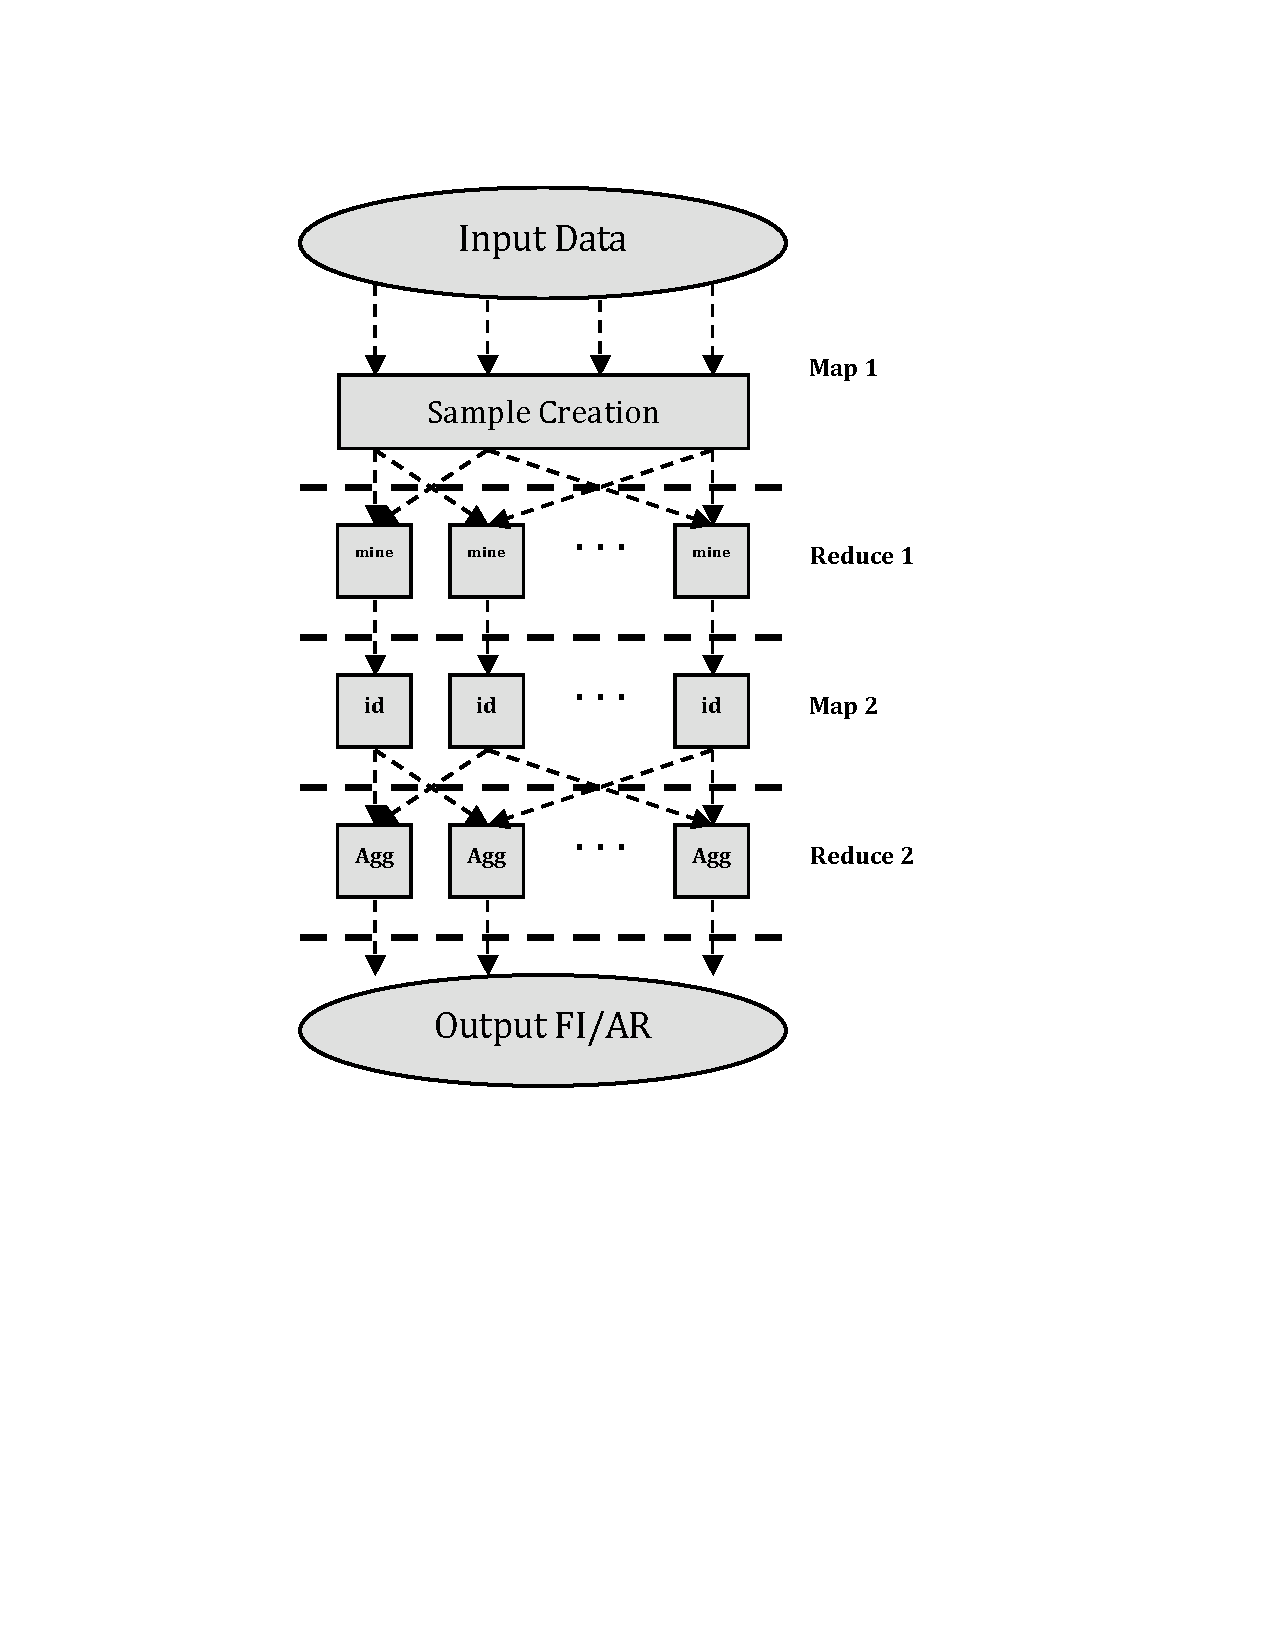
\includegraphics[width=0.3\textwidth]{parma/overview.pdf}
\caption{A system overview of PARMA. Ellipses represent data, squares represent
computations on that data and arrows show the movement of data through the
system.}
\label{fig:parmaoverview}
\end{figure}

  \begin{comment}
  The diagram is broken into 4 main computations which correspond to the
  Map and Reduce phases of the two MapReduce rounds in the algorithm. In
  the Map of Stage 1, a sample is created. In the Reduce of Stage 1, a
  mining algorithm is run on the subset of the sample created in the Map
  phase. This mining algorithm can be either frequent itemset mining or
  association rule mining, and as such is generically labeled mine. In
  the Map phase of Stage 2, the local frequent itemsets are sent to an
  identity mapper, and finally Aggregated in the Stage 2 Reduce to get a
  global set of frequent itemsets or assocation rules, depending on the
  mining algorithm used.
\end{comment}


\paragraph*{Computing $N$ and $w$} From the above discussion it should be clear
that, once $p$, $m$, $\varepsilon$ and $\delta$ have been fixed, there is a
trade-off between $w$ and $N$. In the MapReduce setting, often the most expensive
operation is the movement of data between the mappers and the reducers in the
shuffle phase. In PARMA, the amount of data to be shuffled corresponds to the
sum of the sizes of the samples, i.e., $Nw$, and to the amount of
communication needed in the aggregation stage. This second quantity is dependent
on the number of frequent itemsets in the dataset, and therefore PARMA has no
control over it. PARMA tries to minimize the first quantity when computing $N$ and
$w$ in order to achieve the maximum speed. It is still possible to minimize for
other quantities (e.g. $\varepsilon$ or $\delta$ if they have not been fixed),
but we believe the most effective and natural in the MapReduce setting is the
minimization of the communication.  This intuition was verified in our
experimental evaluation, where communication proved to be the dominant cost. We
can formulate the problem of minimizing $Nw$ as the following Mixed Integer Non
Linear Programming (MINLP) problem:
\begin{itemize}
  \item {\bf Variables:} non-negative integer $N$, real $\phi\in(0,1)$,
  \item {\bf Objective:} minimize $2N/\varepsilon^2 (d+\log(1/\phi))$.
  \item {\bf Constraints:}
    \begin{align}
      &N \le p \label{eq:parmaconstr1}\\
      &\phi \ge e^{-m\varepsilon^2/2 + d} \label{eq:parmaconstr2}\\
      &N(1-\phi)-\sqrt{N(1-\phi)2\log(1/\delta)} \ge N/2 + 1 \label{eq:parmaconstr3}
    \end{align}
\end{itemize}
Note that, because of our requirement {\bf 2)} on $w$, the sample size $w$ is directly
determined by $\phi$ through Lemma~\ref{lem:keythmfi}, so the trade-off is
really between $N$ and $\phi$, while $w$ does not appear in the above problem.
Since $\phi$ is a probability we restrict its
domain to the interval $(0,1)$, but it must also be such that the single sample size
$w$ is at most $m$, as required by {\bf 1)} and expressed by
Constraint~\eqref{eq:parmaconstr2}. The limit to the number of samples $N$ is expressed by
Constraint~\eqref{eq:parmaconstr1}. The last constraint~\eqref{eq:parmaconstr3} is a bit
more technical and the need for it will be evident in the analysis of the
algorithm. Intuitively, it expresses the fact that an itemset must appear in a
sufficiently high fraction (at least 1/2, possibly more) of the collections obtained from the samples in the
first stage in order to be included in the output collection. Due to the integrality constraint on
$N$, this optimization problem is not convex, although when the constraint it is
dropped the feasibility region is convex, and the objective function is convex.
It is then relatively easy and fast to find an integer optimal solution to the
problem using a global MINLP solver like BARON~\cite{baron}. 

%\paragraph{Overview} PARMA builds on a previous work~\cite{RiondatoU12} which
%presented algorithms to probabilistically extract $\varepsilon$-approximations
%of FI's and AR's using a random sample of the dataset, in a sequential setting.
%The size of the sample suggested in~\cite{RiondatoU12} work depends on the
%desidered accuracy and probability of error parameters $\varepsilon$ and
%$\delta$. When extremely accurate approximations are desired with a very low
%probability of error ($\varepsilon$ and $\delta$ are very small), the resulting
%sample may become too large to be easily handled by a single machine. By
%exploiting the parallel/distributed architecture of MapReduce, PARMA allows to
%obtain very high-confidence and extremely accurate approximations by first
%creating and mining a number of smaller samples in parallel using appropriately
%lowered frequency and confidence thresholds. For each sample, the collection
%obtained by mining it is a $(\varepsilon,\varepsilon/2)$-approximation of the
%desired collection of FI's or AR's with probability at least $1-\phi$, where
%$\phi\ge\delta$. In its second phase, PARMA aggregates these collections to
%obtain a single collection to be output. Although it can only offer the same
%analytical guarantees, in practice PARMA can return approximations of higher
%quality than what the sequential approach in~\cite{RiondatoU12} could do, thanks
%to the aggregation of multiple estimations of the frequencies and the
%confidences of the FI's and AR's. The aggregation allows for a decrease in the
%false positives discovery rate in the output collection and in improved accuracy
%in the estimation of the frequencies and of the confidences of FI's and AR's.
%Figure~\ref{fig:parmaoverview} shows a system overview of PARMA. The algorithm is
%described in details in the next few paragraphs.

%\begin{figure}[t]
%\centering
%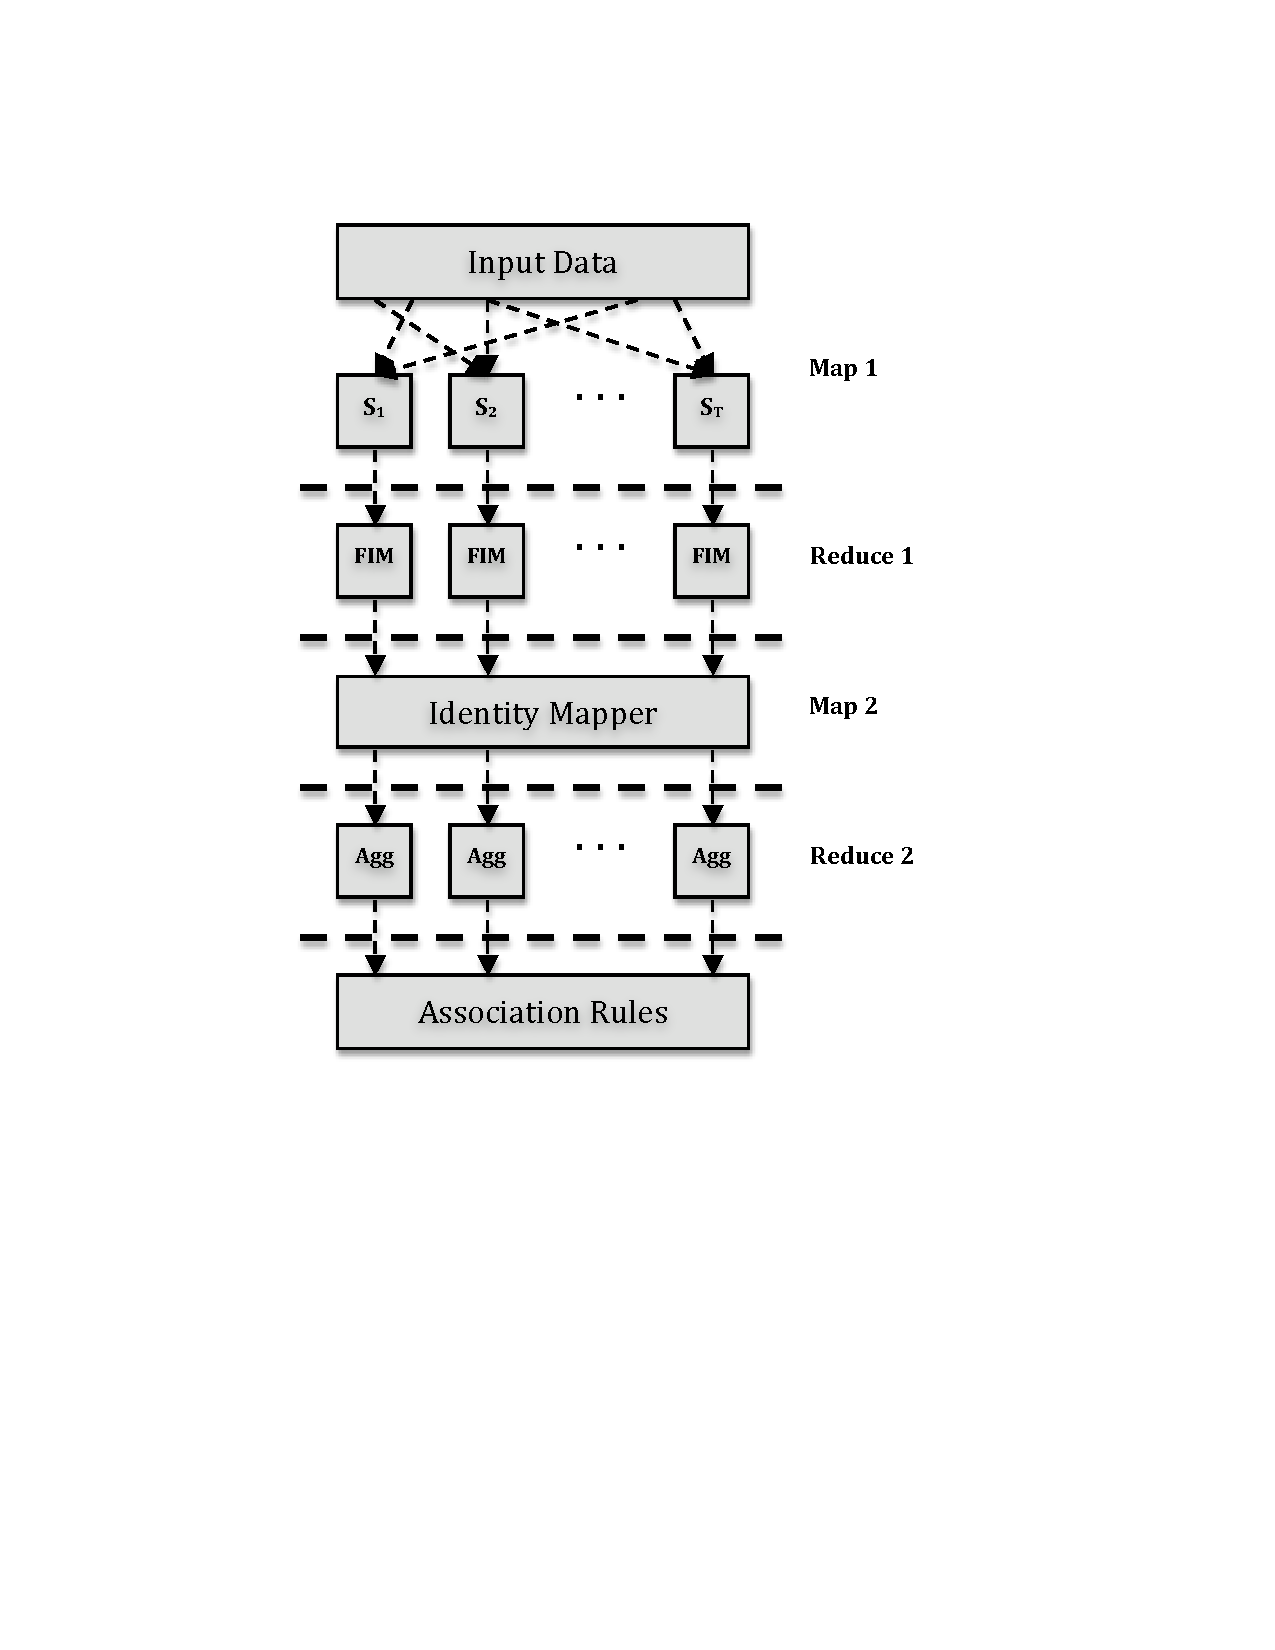
\includegraphics[width=0.45\textwidth]{parmm_overview}
%\caption{A system overview of PARMM.}
%\label{fig:parmaoverview}
%\end{figure}

%\paragraph{Parameters} PARMA has a number of input parameters, in addition
%to the expected parameters describing the ARM task, like the dataset $\Ds$, the
%minimum frequency threshold $\theta$ (or $K$ for Top-$K$ FI's mining) and the
%minimum confidence threshold $\gamma$ (only for mining AR's). The accuracy and
%the probability of error in the output of the algorithm are expressed by the two
%parameters $\varepsilon$ and $\delta$. The algorithm will return an
%$\varepsilon$-approximation of the desired collection of FI's or AR's with
%probability at least $1-\delta$. There are two additional parameters $m$ and $M$
%which control the behaviour of PARMA. They are respectively the maximum sample
%size (in number of transactions) that can be handled by a single machine in the
%MapReduce cluster and the maximum total sample size (i.e. the sum of the single
%sample sizes). The parameters $m$ and $M$ try to capture the computational power
%(more specifically the memory limitations) of the MapReduce cluster running
%PARMA. PARMA will use samples of size $w\le m$ and a number of samples $N$ such
%that $wN \le M$. One last parameter needed by PARMA is $d$,the maximum integer
%such that $\Ds$ has at least $d$ transactions of length at least $d$.

%We denote with $\phi$ the probability that the collection obtained from a
%of the samples is not an $\varepsilon$-approximation to the desired collection.
%For the case of $\FI(\Ds,\Itm,\theta)$, we can express $w$ as function of
%$\phi$, $\varepsilon$, and $d$~\cite{RiondatoU12}: 
%\begin{equation}\label{eq:parmasinglesamplesize}
%w=\frac{2}{\varepsilon^2}\left(d+\log\frac{1}{\phi}\right)
%\end{equation}
%Note how this expression is independent of $\theta$. Similar expressions of $w$
%can be obtained for the case of $\TOPK(\Ds,\Itm,K)$ and
%$\AR(\Ds,\Itm,\theta,\gamma)$~\cite{RiondatoU12}. The values for $\phi$, $w$,
%and $N$ are computed by minimizing the total number of sampled transactions
%$wN$, under some constraints (see below). Note that we will assume that 
%\[ m < \frac{2}{\varepsilon^2}\left(d + \log\frac{1}{\delta}\right)\]
%otherwise we would be able to obtain an $\varepsilon$-approximation with
%probability $1-\delta$ by mining just one sample using Lemma~\ref{lem:keythmfi}.

%\paragraph{Computing $w$ and $N$} One of the goals of PARMA is to minimize the
%amount of data that are sent from mappers to reducers. This is equivalent to minimize
%the total number of sampled transactions $wN$, where $w$ is the size of a single
%sample and $N$ is the number of samples we create. We can formulate the problem
%of minimizing $w$ as the following Mixed Integer Non Linear Programming (MINLP) 
%problem:
%\begin{itemize*}
%  \item {\bf Variables:} non-negative integer $N$, real $\phi\in(0,1)$,
%  \item {\bf Objective:} minimize $2N/\varepsilon^2 (d+\log(1/\phi))$.
%  \item {\bf Constraints:}
%    \begin{align}
%      &\phi \ge e^{-m\varepsilon^2/2 + d} \label{eq:parmaconstr1}\\
%      &2N/\varepsilon^2 (d+\log(1/\phi)) \le M \label{eq:parmaconstr2}\\
%      &N(1-\phi)-\sqrt{N(1-\phi)2\log(1/\delta)} \ge N/2 + 1 \label{eq:parmaconstr3}
%    \end{align}
%\end{itemize*}
%At a first look it may seem that $w$ does not appear in the above optimization
%problem, but it is actually implicitly expressed through $\phi$
%using~\eqref{eq:parmasinglesamplesize}. Since $\phi$ is a probability we define its
%domain to be the interval $(0,1)$, but it must also be such that the single sample size
%$w$ is at most $m$, as expressed by Constraint~\eqref{eq:parmaconstr1}. The upper
%bound to the total number of sampled transaction is expressed by
%Constraint~\eqref{eq:parmaconstr2}. The last constraint is a bit more technical and
%the need for it will be evident in the analysis of the algorithm. Intuitively, it
%expresses the fact that an itemset must appear in the majority of the
%collections obtained from the sample in order to be included in the output
%collection.
%Due to the integrality constraint on $N$, this optimization problem is not
%convex, although when the constraint it is dropped the feasibility region is
%convex, and the objective function is convex. This means that is relatively
%easy to find an integer optimal solution to the problem using a global MINLP
%solver like BARON~\cite{baron}. 

\subsection{Description}
In the following paragraphs we give a detailed description of PARMA. The reader
is also referred to Figure~\ref{fig:parmaoverview} for a schematic representation of
PARMA's data/computational workflow.

\paragraph*{Stage 1: Sampling and Local Mining} Once $\phi$, $w$
and $N$ have been computed, PARMA enters the first MapReduce round to create
the $N$ samples (phase Map 1 in Figure~\ref{fig:parmaoverview}) and mine them (Reduce 1).
We see the input of the algorithm as a sequence
\[
(1,\tau_1),(2,\tau_2),\cdots,(|\Ds|,\tau_{|\Ds|}),\]
where the $\tau_i$ are transactions in $\Ds$.
In the Map phase, the input of the {\bf map} function is a pair $(tid, \tau)$, where
$tid$ is a natural from $1$ to $|\Ds|$ and $\tau$ is a transaction in $\Ds$. The
map function produces in output a pair $(i,(\ell^{(i)}_\tau,\tau))$ for each
sample $\Sam_i$ containing $\tau$. The value $\ell^{(i)}_\tau$ denotes the
number of times $\tau$ appears in $\Sam_i$, $1\le i \le N$. We use random sampling
with replacement and ensure that all samples have size $w$, i.e.,
$\sum_{\tau\in\Ds}\ell^{(i)}_\tau=w$, $\forall i$. This is done by computing
(serially) how many transactions each mapper must send to each sample. In the
Reduce phase, there are $N$ reducers, with associated key $i$, $1\le i \le N$.
The input to reducer $i$ is $(i,\Sam_i)$, $1\le i\le N$. Reducer $i$ mines the
set $\Sam_i$ of transactions it receives using an exact sequential mining
algorithm like Apriori or FP-Growth and a lowered minimum frequency threshold
$\theta'=\theta-\varepsilon/2$ to obtain
$\mathcal{C}_i=\FI(\Sam_i,\Itm,\theta')$. For each itemset $A\in\mathcal{C}_i$
the Reduce function outputs a pair $(A,
(f_{\Sam_i}(A),[f_{\Sam_i}(A)-\varepsilon/2,f_{\Sam_i}(A)+\varepsilon/2])$.

\paragraph*{Stage 2: Aggregation} In the second round of MapReduce, PARMA
aggregates the result from the first stage to obtain a
$\varepsilon$-approximation to $\FI(\Ds,\Itm,\theta)$ with probability at least
$1-\delta$. The Map phase (Map 2 in Figure~\ref{fig:parmaoverview}) is just the identity
function, so for each pair 
\[(A,
(f_{\Sam_i}(A),[f_{\Sam_i}(A)-\varepsilon/2,f_{\Sam_i}(A)+\varepsilon/2])\]
in the input the same pair is produced in the output. In the Reduce phase (Reduce 2) there
is a reducer for each itemset $A$ that appears in at least one of the
collections $\mathcal{C}_j$ (i.e., $\forall A$ such that there is a
$\mathcal{C}_j$ containing a pair related to $A$). The reducer receives as input
the itemset $A$ and the set $\mathcal{F}_A$ of pairs
\[
(f_{\Sam_i}(A),[f_{\Sam_i}(A)-\varepsilon/2,f_{\Sam_i}(A)+\varepsilon/2])\]
for the samples $\Sam_i$ such that $A\in\mathcal{C}_i$.
Now let
\begin{equation}\label{eq:parmaRdef}
R = N(1-\phi)-\sqrt{N(1-\phi)2\log(1/\delta)}.
\end{equation}
The itemset $A$ is declared
\emph{globally frequent} and will be present in the output if and only if
$|\mathcal{F}_A| \ge R$. If this is the case, PARMA computes, during the Reduce
phase of the second MapReduce round, the estimation $\tilde{f}(A)$ for the
frequency $f_\Ds(A)$ of the itemset $A$ in $\Ds$ and the confidence interval
$\mathcal{K}_A$. The computation for $\tilde{f}(A)$ proceeds as follows. Let
$[a_A,b_A]$ be the \emph{shortest} interval such that
there are at least $N-R+1$ elements from $\mathcal{F}_A$ that belong to this
interval. The estimation $\tilde{f}(A)$ for the frequency $f_\Ds(A)$ of the
itemset $A$ is the central point of this interval:
\[ \tilde{f}(A)=a_A+\frac{b_A-a_A}{2}\]
The confidence interval $\mathcal{K}_A$ is defined as
\[ \mathcal{K}_A=\left[a_A-\frac{\varepsilon}{2},b_A+\frac{\varepsilon}{2}\right].\]
The output of the reducer assigned to the itemset $A$ is \[(A,(\tilde{f}(A),\mathcal{K}_A)).\]
The output of PARMA is the union of the outputs from all reducers.

\subsection{Analysis}
We have the following result:
\begin{lemma}\label{lem:multiepsapprox}
 The output of the PARMA is an $\varepsilon$-approximation of
 $\FI(\Ds,\Itm,\theta)$ with probability at least $1-\delta$.
\end{lemma}

\begin{proof}
  For each sample $\Sam_i$, $1\le i\le N$ we define a random variable $X_i$ that
  takes the value $1$ if $\mathcal{C}_i=\FI(\Sam_i,\Itm,\theta')$ is a
  $(\varepsilon,\varepsilon/2)$-approximation of $\FI(\Ds,\Itm,\theta)$, $X_i=0$
  otherwise. Given our choices of $w$ and $\theta'$, we can apply
  Lemma~\ref{lem:keythmfi} and have that $\Pr(X_i=1)\ge 1-\phi$. Let
  $Y=\sum_{r=1}^N X_r$ and let $Z$ be a random variable with binomial
  distribution with parameters $N$ and $1-\phi$. For any constant $Q<N(1-\phi)$ we have
  \[
  \Pr(Y\le Q)\le\Pr(Z\le Q)\le e^{-N(1-\phi)(1-\frac{Q}{N(1-\phi)})^2/2},
  \]
  where the last inequality follows from an application of the Chernoff
  bound~\cite[Chap.~4]{MitzenmacherU05}.
  We then have, for our choice of $\phi$ and $N$ and for $Q=R$
  (defined in Eq.~\eqref{eq:parmaRdef}), that with probability at least $1-\delta$,
  at least $R$ of the collections $\mathcal{C}_i$ are
  $(\varepsilon,\varepsilon/2)$-approximations of $\FI(\Ds,\Itm,\theta)$. Denote
  this event as $\mathcal{G}$. For the rest of the proof we will assume that
  $\mathcal{G}$ indeed occurs.

  Then $\forall A\in\FI(\Ds,\Itm,\theta)$, $A$ belongs to at least $R$ of the
  collections $\mathcal{C}_i$, therefore a triplet
  $(A,\tilde{f}(A),\mathcal{K}_A)$ will be in the output of the algorithm. This
  means that Property 1 from Def.~\ref{def:parmaeapproxfi} holds. 

  Consider now any itemset $B$ such that $f_\Ds(B)<\theta-\varepsilon$. By
  definition of $(\varepsilon,\varepsilon/2)$-approximation we have that $B$ can
  only appear in the collections $\mathcal{C}_i$ that are not
  $(\varepsilon,\varepsilon/2)$-approximations. Given
  that $\mathcal{G}$ occurs, then there are at most  $N-R$ such collections. But
  from Constraint~\eqref{eq:parmaconstr3} and the definition of $R$
  in~\eqref{eq:parmaRdef}, we have that $N-R< R$, and therefore $B$ will not be
  present in the output of PARMA, i.e.~Property 2 from Def.~\ref{def:parmaeapproxfi} holds.

  Let now $C$ be any itemset in the output, and consider the interval
  $S_C=[a_C,b_C]$ as computed by PARMA. $S_C$ contains at least $N-R+1$ of
  the $f_{\Sam_i}(C)$, otherwise $C$ would not be in the output. By our
  assumption on the event $\mathcal{G}$, we have
  that at least $R$ of the $f_{\Sam_i}(C)$'s are such that
  $|f_{\Sam_i}(C)-f_\Ds(C)|\le\varepsilon/2$. Then there is an index $j$ such
  that $|f_{\Sam_j}(C)-f_\Ds(C)|\le\varepsilon/2$ and such that
  $f_{\Sam_j}(C)\in S_C$.
  Given also that $f_{\Sam_j}(C)\ge a_C$, then $f_\Ds(C)\ge
  a_C-\varepsilon/2$, and analogously, given that $f_{\Sam_j}(C)\le b_C$, then
  $f_\Ds(C)\le b_C+\varepsilon/2$. This means that
  \begin{equation}\label{eq:parmasingleepsapproxinterval}
    f_\Ds(C)\in
    \left[a_C-\frac{\varepsilon}{2},
    b_C+\frac{\varepsilon}{2}\right]=\mathcal{K}_C,
  \end{equation}
  which, together with the fact that $\tilde{f}_C\in\mathcal{K}_C$ by
  construction, proves Property 3.b from Def.~\ref{def:parmaeapproxfi}.
  We now give a bound to $|S_C|=b_C-a_C$. From our
  assumption on the event $\mathcal{G}$, there are (at least) $R$ values
  $f_{\Sam_i}(C)$ such that $|f_{\Sam_i}(C)-f_\Ds(C)|\le\varepsilon/2$, then the
  interval $[f_\Ds(C)-\varepsilon/2,f_\Ds(C)+\varepsilon/2]$ contains (at least)
  $R$ values $f_{\Sam_i}(C)$. Its length $\varepsilon$ is an upper bound to
  $|S_C|$. Then the length of the interval
  $\mathcal{K}_C=[a_C-\varepsilon/2,b_C+\varepsilon/2]$ is at most
  $2\varepsilon$, as requested by Property 3.c from
  Def.~\ref{def:parmaeapproxfi}. From this, from ~\eqref{eq:parmasingleepsapproxinterval}, and
  from the fact that $\tilde{f}(C)$ is the center of this interval we have
  $|\tilde{f}(C)-f_\Ds(C)|\le\varepsilon$, i.e., Property 3.a from
  Def.~\ref{def:parmaeapproxfi} holds.
\end{proof}

\subsection{Top-K Frequent Itemsets And Association Rules}\label{sec:parmaeapproxtopk}
The above algorithm can be easily adapted to computing, with probability at
least $1-\delta$, $\varepsilon$-approximations to $\TOPK(\Ds,\Itm,K)$ and to
$\AR(\Ds,\Itm,\theta,\gamma)$. The main difference is in the formula to compute
the sample size $w$ (Lemma~\ref{lem:keythmfi}), and in the process
to extract the local collections from the samples. The case of top-$K$ is
presented in~\cite{RiondatoU12} and is a minor modification of
Lemma~\ref{lem:keythmfi}, while for the association rule case we can use
Lemma~\ref{lem:keythmar}. These are minimal changes to the version of
PARMA presented here, and the modified algorithms guarantee the same levels of
accuracy and confidence.

%main difference is in the formula to compute sample size $w$
%(Eq.~\eqref{eq:parmasinglesamplesize}, which in this case is set to $w=8(d+\log
%1/\phi)/varepsilon^2$, and in the work done by the reducers in the
%first phase: using the algorithm presented in~\cite[Lemma 3]{RiondatoU12}, each
%reducer $r$ computes, with probability at least $1-\phi$, a collection
%$\mathcal{C}_r$ such that if we see $\TOPK(\Ds,\Itm,K)$ as
%$\FI(\Ds,\Itm,f^{(K)}_\Ds)$, $\mathcal{C}_r$ is a
%$(\varepsilon,\varepsilon/2)$-approximation to $\FI(\Ds,\Itm,f^{(K)}_\Ds)$. The
%collections $\mathcal{C}_i$'s are then aggregated in the second MapReduce round
%in the same way as for the case of FI's  described in the previous section. This
%result is formulated in the following Lemma, whose proof will be included in the
%full version of the paper. 
%\begin{lemma}
%   The output of the algorithm is an $\varepsilon$-approximation of
%   $\TOPK(\Ds,\Itm,K)$ with probability at least $1-\delta$.
%\end{lemma}
%
%\subsection{Association Rules}\label{sec:parmaeapproxar}
%The above algorithm can be easily adapted to computing, with probability at
%least $1-\delta$, an $\varepsilon$-approximation to
%$\AR(\Ds,\Itm,\theta,\gamma)$. The main differences are again in how to compute
%the sample size $w$ (see Lemma~\ref{lem:keythmar}) and in the work done by the
%reducers in the first phase. Using the algorithm presented in~\cite[Lemma
%6]{RiondatoU12}, each reducer $r$ computes a collection $\mathcal{C}_r$ such
%that $\mathcal{C}_r$ is a $(\varepsilon,\varepsilon/2)$-approximation to
%$\AR(\Ds,\Itm,\theta,\gamma)$  with probability at least
%$1-\phi$, The collections $\mathcal{C}_r$ are then aggregated in the second
%MapReduce phase as described in the previous section, with the only addition of
%computing an estimate $\tilde{g}(W)$ for the confidence $g_\Ds(W)$ of each
%association rule $W$ in the output, and an interval $\mathcal{J}(W)$. This can be
%done exactly in the same way as computing the estimate $\tilde{f}(W)$ for the
%frequency $f_\Ds(W)$ and the corresponding interval $\mathcal{K}(W)$. The
%properties of the output are formulated in the following Lemma, whose proof will
%be included in the full version of the paper.
%\begin{lemma}
%   The output of the algorithm is an $\varepsilon$-approximation of
%   $\AR(\Ds,\Itm,\theta,\gamma)$ with probability at least $1-\delta$.
%\end{lemma}
%

\section{Implementation} 
\label{sec:parmadesign} 
The entire PARMA algorithm has been written as a Java library for
Hadoop, the popular open source implementation of MapReduce. Because all
experiments were done using Amazon Web Service (AWS) Elastic MapReduce,
the version of Hadoop used was 0.20.205, the highest supported by AWS.
The use of Java makes possible future integration with the Apache Mahout
parallel machine learning library~\cite{Mahout}. Mahout also includes an
implementation of PFP~\cite{LiWZZC08} that we used for our evaluation of
PARMA.

In PARMA, during the mining phase (i.e. during the reducer of stage 1),
any frequent itemset or association rule mining algorithm can be used.
We wanted to compare the performances of PARMA against PFP which only
produces frequent itemsets, therefore we chose to use a frequent itemset
mining algorithm instead of an association rule mining algorithm. Again,
this choice was merely for ease of comparison with existing parallel
frequent itemset mining algorithms as no such algorithms for association
rule mining exist. While there are many frequent itemset mining
algorithms available, we chose the FP-growth implementation provided
by~\cite{Fp}. We chose FP-growth due to its relative performance
superiority to other Frequent Itemsets mining algorithms. Additionally,
since FP-growth is the algorithm that PFP has parallelized and uses
internally, the choice of FP-growth for the mining phase in PARMA is
appropriate for a more natural comparison.

We also compare PARMA against the naive distributed counting algorithm
(DistCount) for computing frequent itemsets. In this approach, there is
only a single MapReduce iteration. The map breaks a transaction $\tau$
into its powerset $\mathcal{P}(\tau)$ and emits key/value pairs in the
form $(A, 1)$ where $A$ is an itemset in $\mathcal{P}(t)$. The reducers
simply count how many pairs they receive for each itemset $A$ and output
the itemsets with frequency above the minimum frequency threshold. This
is similar to the canonical wordcount example for MapReduce. However,
because the size of the powerset is exponential in the size of the
original transaction (specifically $2^{|\tau|}$, where $|\tau|$ denotes
the number of items in a given transaction), this algorithm incurs
massive network costs, even when combiners are used. This is very similar to the
algorithms presented in~\cite{CryansRC10,LiZ11,YangLF10}. We have built our own
implementation of DistCount in Java using the Hadoop API.

\section{Experimental evaluation}
\label{sec:parmaeval}

We evaluate the performance of PARMA using Amazon's Elastic
MapReduce platform. We used instances of type \emph{m1.xlarge}, which
contain roughly 17GB of memory and 6.5 EC2 compute units.
For data, we created artificial dataset using the synthetic data
generator from~\citep{ARTool}. This implementation is based on the
generator described in~\citep{AgrawalS94}, which can be parameterized to generate a wide
range of data. We used two distinct sets of parameters to generate the
datasets: the first set, shown in Table~\ref{tab:param1}, for the experiments
comparing PARMA and the distributed counting algorithm
(DistCount), and the second set, shown in Table~\ref{tab:param2},
for the experiments comparing PARMA and PFP.
The parameters were
chosen to mimic real-world datasets on which PARMA would be run. For a
full description of the relevant parameters, we refer the reader to
\citep{AgrawalS94}.  
The reason we needed two distinct datasets is that DistCount did not scale to
the larger dataset sizes,  as the amount of data it generates in the map phase
grows exponentially with the length of the individual transactions in the
dataset.  We found that DistCount would run out of memory using datasets with
longer transactions, and we had to generate datasets with both shorter and less
transactions for its comparisons. 
%This is a strong
%testament to the lack of scalability of the distributed counting
%algorithm.  

Because PARMA is an approximate algorithm, the choice of accuracy
parameters $\varepsilon$ and $\delta$ are important, as is $\theta$,
the minimum frequency at which itemsets were mined. In all of our
experiments, $\varepsilon = 0.05$ and $\delta = 0.01$. This means that
the collection of itemsets mined by PARMA will be an absolute 0.05-close
approximation with probability 0.99. In practice, we show later that the results
are much more accurate than what this. For all experiments other than the
minimum frequency performance comparison in Figure \ref{fig:parmafrequency} and for
the accuracy comparison in Figures~\ref{fig:parmaabsfreqerr}
and~\ref{fig:parmaconfintwidth}, $\theta$ was kept constant at 0.1.

We focus on three main aspects in the experimental analysis of PARMA. First is the runtime
analysis. In this set of experiments we compare PARMA to PFP and DistCount using several
different datasets of varying size and mined with varying minimum frequency thresholds. We
then break down the runtime of PARMA into the map, reduce and shuffle phases of each of
the two stages. This demonstrates which parts of the algorithm have runtimes that increase
as the data size grows and which parts are relatively data independent. The second aspect
is speedup, to show the scalability of our algorithm. In these experiments, data and
cluster size are varied to determine how PARMA scales. Finally, because the output of
PARMA is an absolute $\varepsilon$-close approximation of the real set of frequent itemsets, we provide
an accuracy analysis to verify that our results are indeed within the desired quality
bounds.

\begin{table}[tb] \centering
\begin{tabular}{ l  r } \hline number of items & 1000 \\ 
average transaction length & 5 \\ 
average size of maximal potentially large itemsets & 5 \\ 
number of maximal potentially large itemsets & 5 \\
correlation among maximal potentially large itemsets & 0.1 \\
corruption of maximal potentially large itemsets & 0.1 \\ \hline
\end{tabular}
  \caption{Parameters used to generate the datasets for the runtime comparison between 
  DistCount and PARMA in Figure \ref{fig:parmaperformance}.}
  \label{tab:param1}
\end{table}

\begin{table}[tb] \centering
\begin{tabular}{ l  r } 
\hline 
number of items & 10000 \\ 
average transaction length & 10 \\ 
average size of maximal potentially large itemsets & 5 \\ 
number of maximal potentially large itemsets & 20 \\
correlation among maximal potentially large itemsets & 0.1 \\
corruption of maximal potentially large itemsets & 0.1 \\ 
\hline
\end{tabular}
  \caption{Parameters used to generate the datasets for the runtime comparison
  between PFP and PARMA in Figure \ref{fig:parmaperformance}.}
  \label{tab:param2}
\end{table}
%Due to space limitations, we do not report the results of the experiments to
%evaluate the performances of PARMA as the parameters of the optimization problem change.

\subsection{Performance analysis} 

For the performance analysis of PARMA, we analyze the relative
performance against two exact FIM algorithms on MapReduce,
\emph{DistCount} and \emph{PFP}, on a cluster of 8 nodes. We also provide a breakdown of the costs
associated with each stage of PARMA.


Figure~\ref{fig:parmaperformance} (top) shows the comparison
between PARMA and DistCount.
As discussed previously, due to
limitations in the scalability of DistCount, we were unable to test on
the larger datasets, so the smaller datasets were generated using
parameters from Table \ref{tab:param1}. 
For DistCount,
longer itemsets affect runtime the most, as
the number of key/value pairs generated from each transaction is
exponential in the size of the transaction. This is not to say that more
transactions does not affect runtime, just that the length of those
transactions also has a significant impact. Because of this, it is
possible to have datasets with fewer transactions but with more ``long''
transactions that take longer to mine. This effect is seen in the first
three datasets (1-3 million). Even though the number of transactions
significantly increases, the relative length of the longest transactions
was actually longer in the 1 million transaction dataset. Indeed, upon
further inspection, we found that the 1 million transaction dataset had
25 transactions over 20 items in length, while the 2 and 3 million
transaction dataset had less than 15. 
Of course, since these datasets
were generated independently and with the same parameters,
this was purely by chance. However, as the number of transactions continues to
increase, the exponential growth in the number of intermediate key/value
pairs is seen by the sharp increase in runtime. While we tried to test
with a dataset with 6 million transaction, DistCount ran out of memory.
The lack of ability to handle either long individual transactions or a
large number of transactions in a dataset limits DistCount's
real-world applicability. The runtime of PARMA is significantly faster
than that of DistCount and, more importantly, nearly constant across
dataset sizes. The reasons for this will be discussed in detail later.

\begin{figure}[htb]
  \centering
    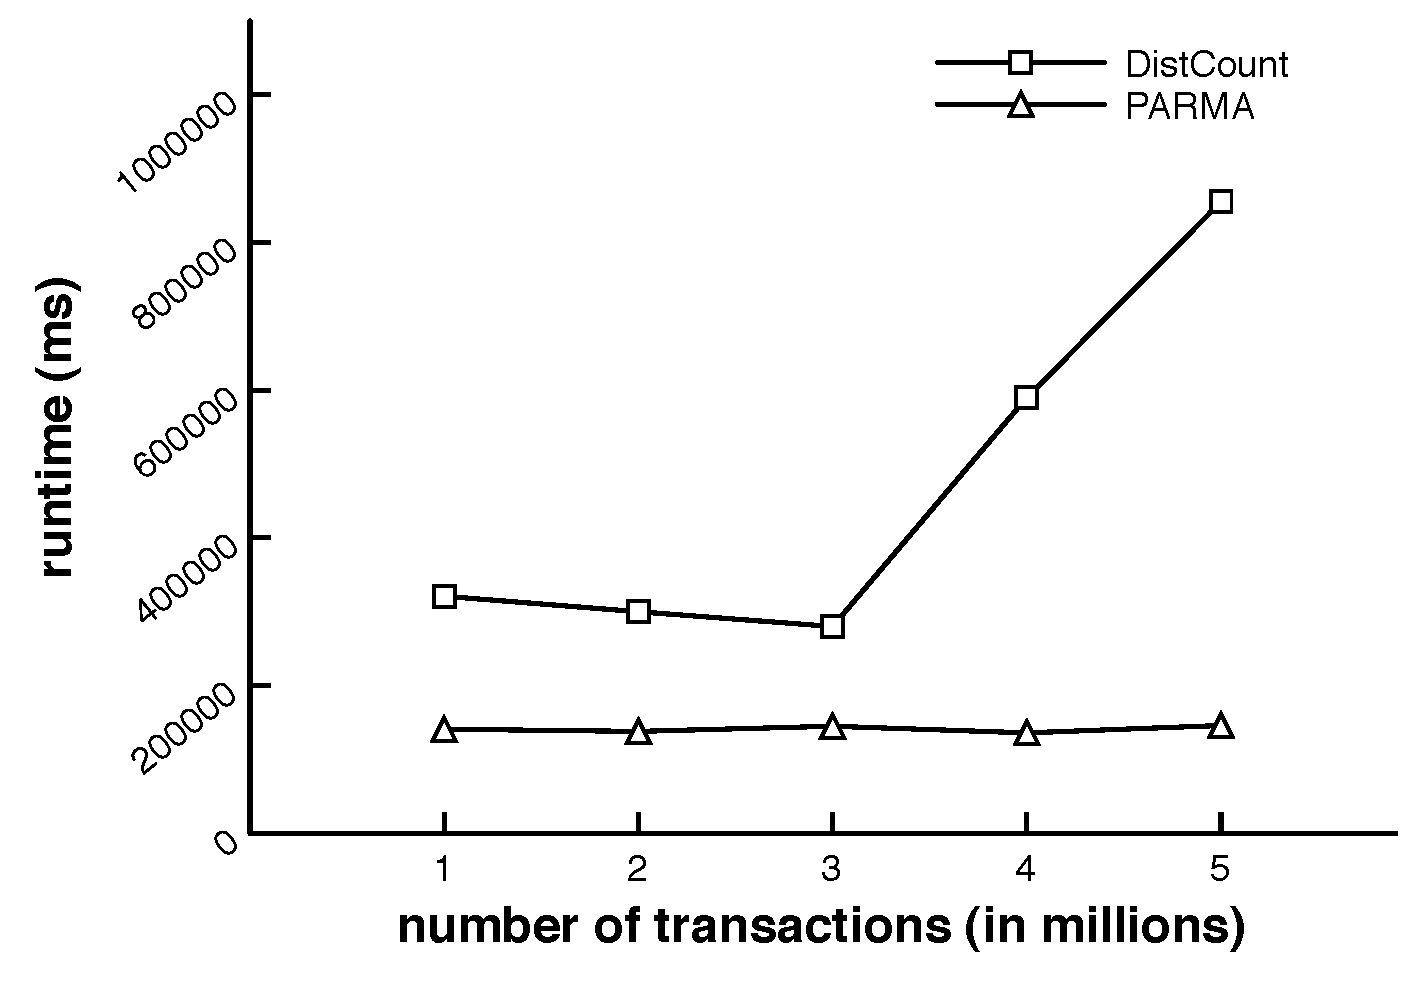
\includegraphics[width=0.49\textwidth]{parma/distributed_counting}
    \hfill
    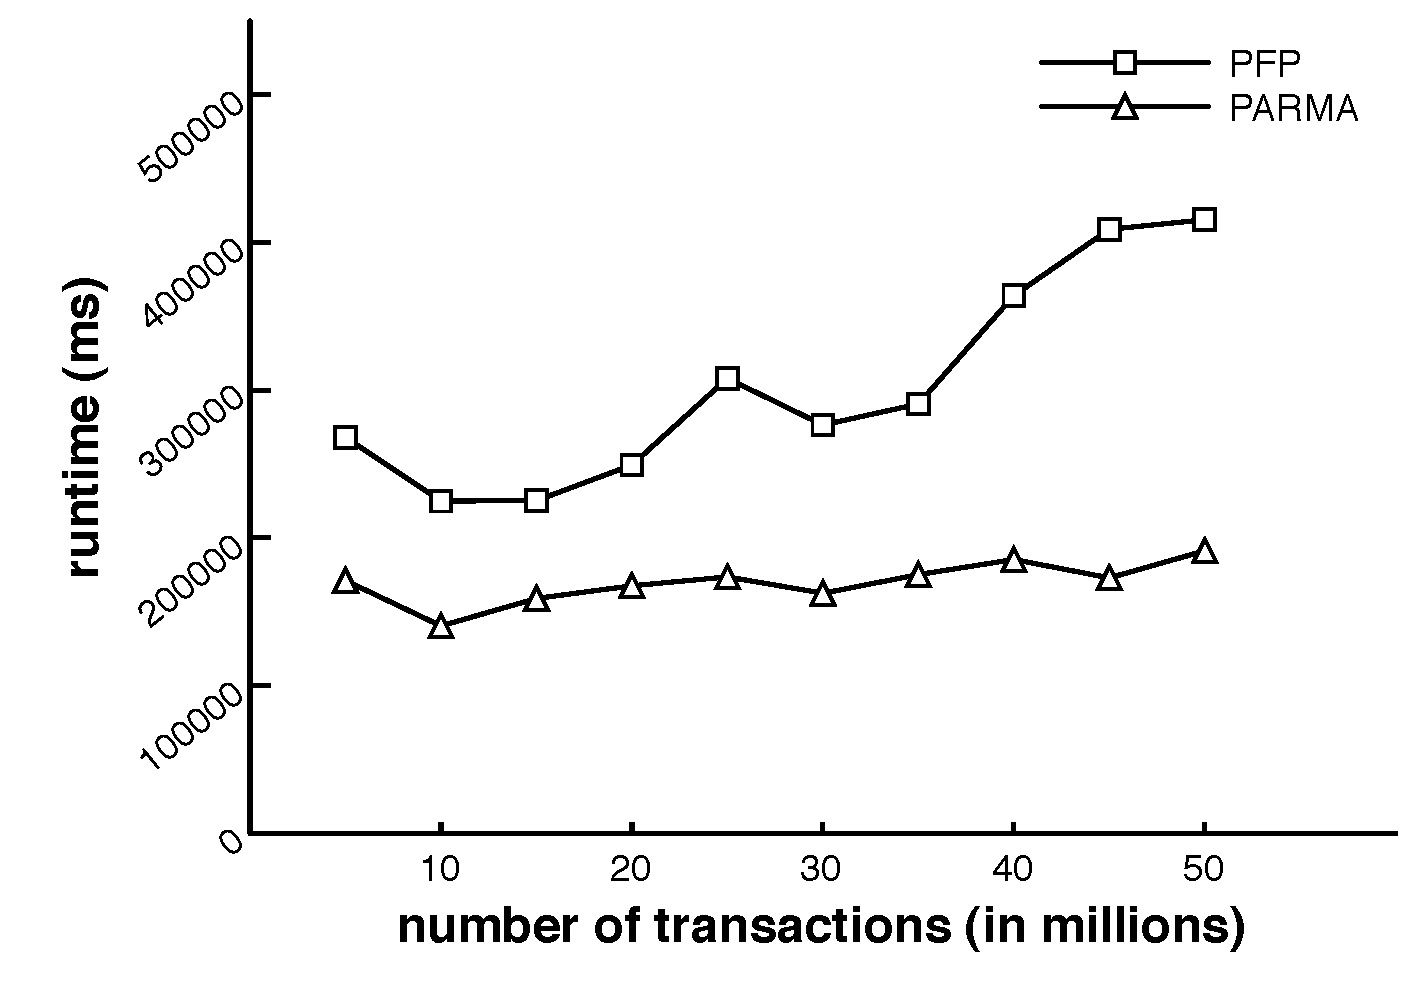
\includegraphics[width=0.49\textwidth]{parma/performance}
  \caption{A runtime comparison of PARMA with DistCount and PFP.}
\label{fig:parmaperformance}
\end{figure}

For the performance comparison with PFP, 10 datasets were generated
using parameter values from Table \ref{tab:param2} and ranging in size
from 10 to 50 million transactions.
The results are shown in
Figure~\ref{fig:parmaperformance} (bottom).
  For every dataset tested, PARMA was able
to mine the dataset roughly 30-55\% faster than PFP. The reason for the
relative performance advantage of PARMA is twofold. The first (and
primary) reason is that for larger datasets the size of the dataset that
PARMA has sampled (and mined) is staying the same, whereas PFP is mining
more and more transactions as the dataset grows. The second reason is
that as the dataset grows, PFP is potentially duplicating more and more
transactions as it assigns transactions to groups. A transaction that
belongs to multiple groups is sent to multiple reducers, resulting in
higher network costs.

The most important aspect of the comparison of PFP to PARMA is that the
runtimes as data grows are clearly diverging due to the reasons
discussed above. While 50 million transactions is very sizable, it is
not hard to imagine real-world datasets with transactions on the order
of billions. Indeed, many point-of-sale datasets would easily break this
boundary. In these scenarios a randomized algorithm such as PARMA would
show increasing performance advantages over exact algorithms such as any
of the standard non-parallel algorithms or PFP, which must mine the
entire dataset. At that scale, even transmitting that data over the
network (several times in the case of PFP) would become prohibitive.

To understand the performance of PARMA it is important to analyze the
runtimes at each of the various stages in the algorithm. To do this, we
have implemented runtime timers at very fine granularities throughout
our algorithm. The timers' values are written to Hadoop job logs for
analysis. This breakdown allows us to not only analyze the overall
runtime, but also the sections of the algorithm whose runtimes are
affected by an increase in data size. In Figure \ref{fig:parmabreakdown1}, a
breakdown of PARMA runtimes is shown for each of the six segments of the
algorithm, which include a map, shuffle and reduce phase for each of the
two stages. 
Due to space limitations, we only show the breakdown for a subset of
the datasets we tested. We observed the same patterns for all datasets.
This breakdown demonstrates several interesting aspects of
PARMA. First, the cost of the mining local frequent itemsets (stage 1,
reduce) is relatively constant. For many frequent itemset mining
implementations, this cost will grow with the size of the input. This is
not the case in PARMA, because local frequent itemset mining is being
done on constant-sized sample of the input. Indeed another interesting
observation, as expected, is that the only cost that increases as sample
size increases is the cost of sampling (stage 1, map). This is because
in order to be sampled the input data must be read, so larger input data
means larger read times. In practice, this cost is minimal and
grows linearly with the input, hence it will never be prohibitive,
especially considering all other current algorithms must read the entire
input data at least once, and in many cases multiple times. 

There is one outlier in the graph, which is the dataset with 5 million
transactions. Because each dataset was independently generated, it is
possible for a dataset to have a larger number of frequent itemsets than
other datasets, even if it has less transactions. This is the case with
the 5 million transaction dataset, which takes longer to run mine for both PARMA and PFP
due to the relatively greater number of frequent itemsets. 

\begin{comment}
To see that this is indeed what is
happening, we refer again to Figure \ref{fig:parmabreakdown1}. As expected,
the sample generation phase (stage 1, map) is smaller relative to the
larger datasets. However, the local frequent itemset mining phase (stage
1, reduce) is longer than any of the larger datasets. This is because
there are more frequent itemsets in that dataset. This can also be seen
in the relatively larger shuffle phase of stage 2, which is in charge of
sending all equivalent local frequent itemsets to the same reducer for
aggregation. Because there are more local itemsets present, this shuffle
stage is larger than for the other datasets. Because the same dataset
was used for the runtime of analysis of PFP and PARMA, and the overall
runtimes of both should increase in a dataset with more frequent
itemsets, we should see a higher runtime on the 5 million transaction
dataset for PFP relative to its the other datasets, which is indeed the
case. The runtime of PFP increases with both the size of the dataset as
well as the number of frequent itemsets present, but it is not until a
dataset of 25 million transactions that the runtime exceeds the runtime
for the 5 million transaction dataset. This outlier is not a flaw with
PARMA or PFP, but is a result of one of the inherent aspects of frequent
itemset mining: it takes longer to mine datasets with more frequent
itemsets.
\end{comment}

\begin{figure}[htb]
\centering
    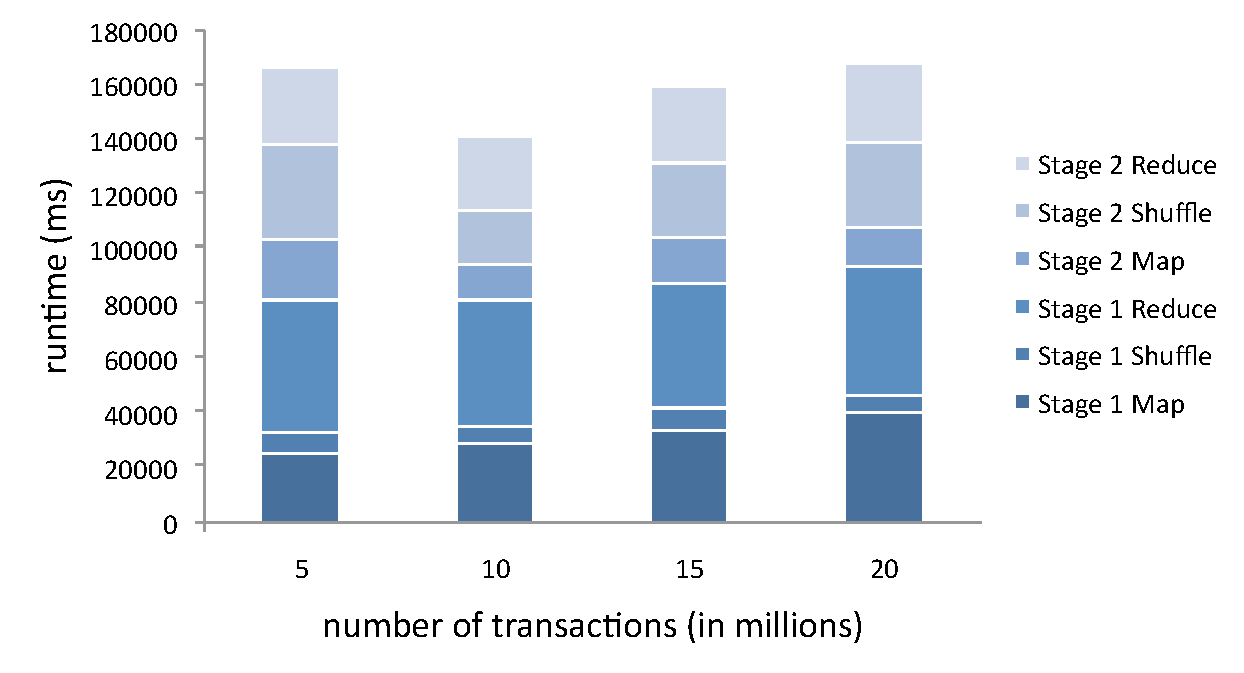
\includegraphics[width=0.75\textwidth]{parma/breakdown1}
  \caption{A comparison of runtimes of the map/reduce/shuffle phases
of PARMA, as a function of number of transactions. Run on
an 8 node Elastic MapReduce cluster.}
\label{fig:parmabreakdown1}
\end{figure}

\begin{figure}[htb]
  \centering
    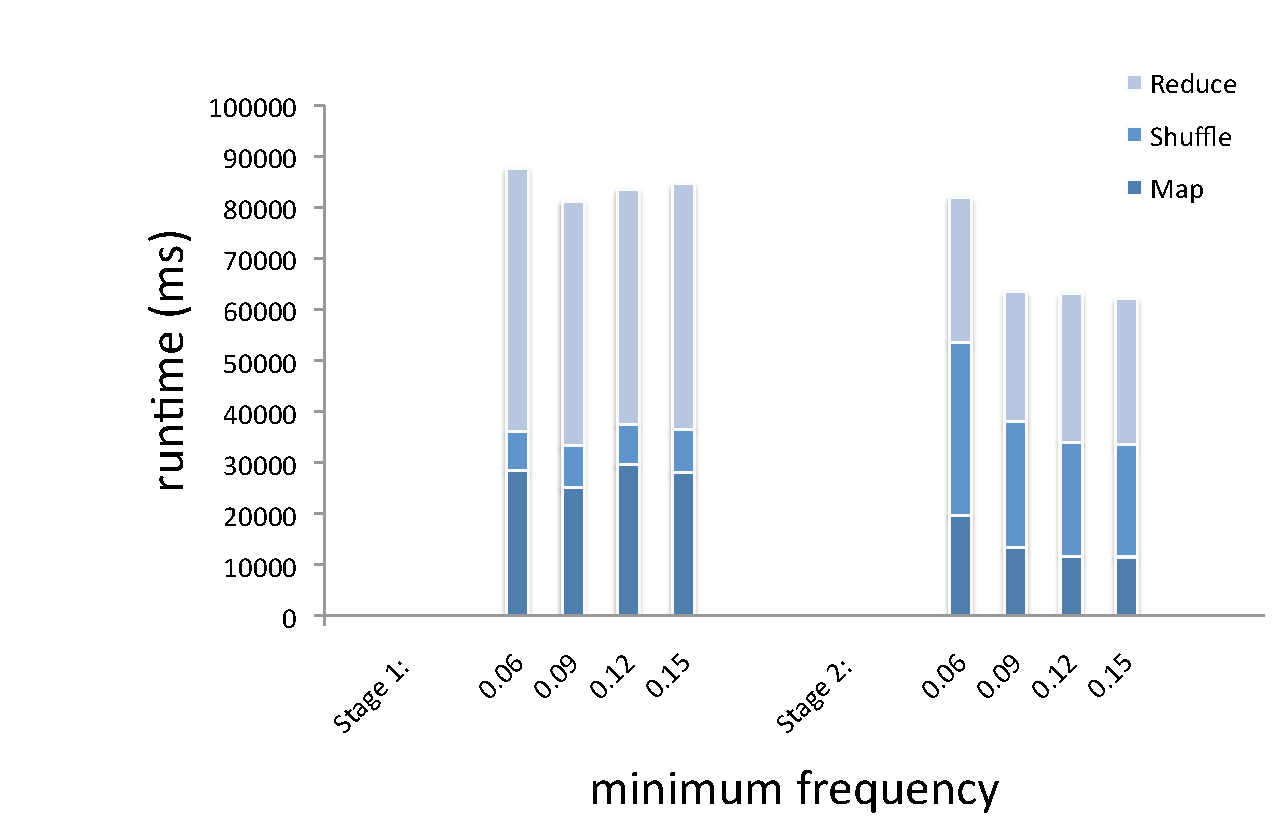
\includegraphics[width=0.75\textwidth]{parma/frequency}
  \caption{A comparison of runtimes of the map/reduce/shuffle phases
of PARMA, as a function of minimum frequency. Clustered by stage. Run
on an 8 node Elastic MapReduce cluster.}
\label{fig:parmafrequency}
\end{figure}

\begin{comment}
In Figure \ref{fig:parmabreakdown2}, a breakdown of total runtimes is shown
clustered by stage. In this view, it is apparent that most of the
phases of the algorithm are nearly constant across data sizes. The
obvious increase is the map of stage 1, which was discussed
above. Another slight runtime increase as data increases occurs in the
shuffle phase of stage 2. Because there are more transactions in the
larger datasets, there will be more frequent itemsets on average. In
stage 2, an identity mapper sends each frequent itemset to the
appropriate reducer for counting. Thus, all this data is being moved
across the network, which is manifested in the shuffle phase of stage
2. The more frequent itemsets, the more data there is to shuffle
across the network, which results in longer runtimes. Also, in
Figure~\ref{fig:parmabreakdown2} we once again notice that the 5 million
transaction dataset is an outlier. The longer than expected phase is
the shuffle phase of stage 2, which again suggests that this dataset
took longer to mine because more frequent itemsets were found.
\begin{figure}[htb]
  \centering
    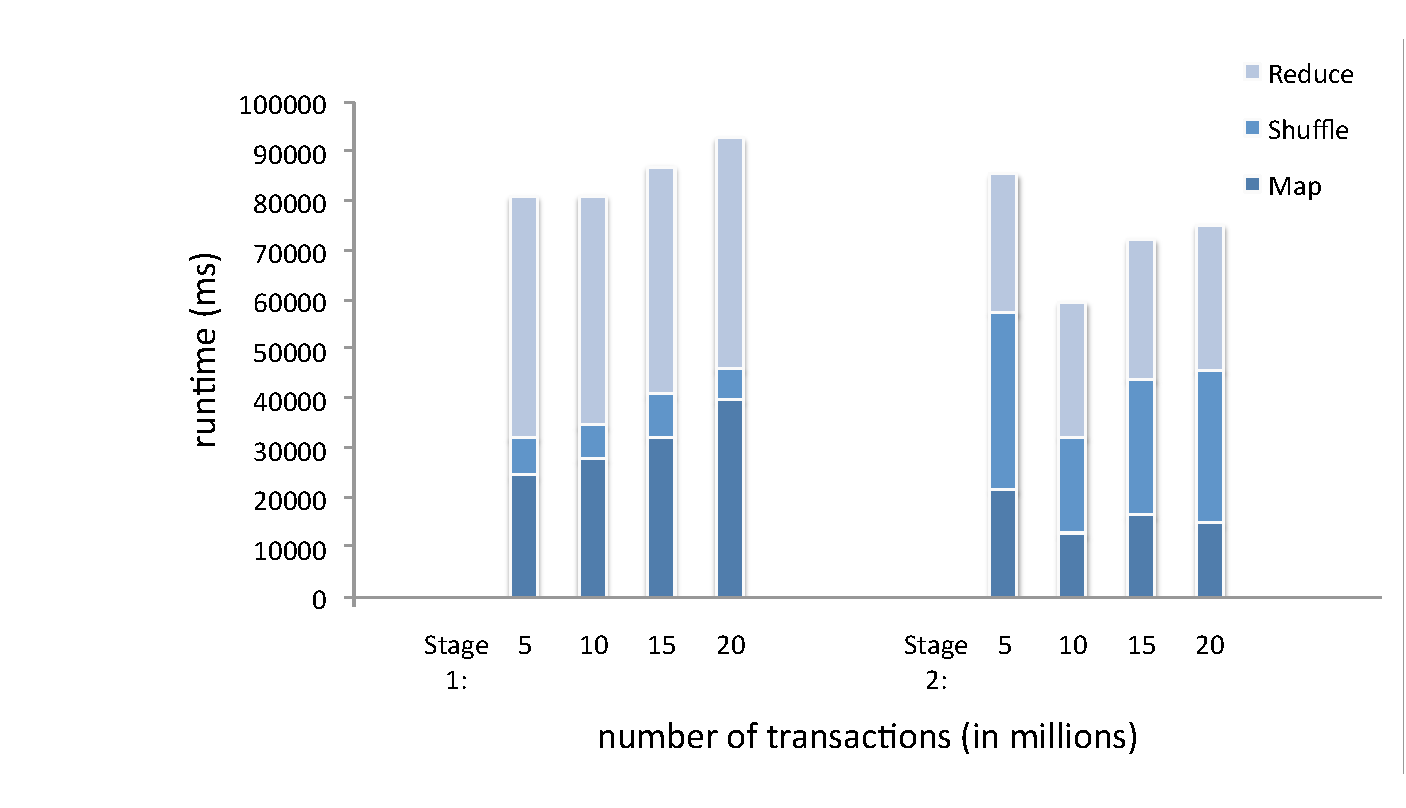
\includegraphics[width=0.4\textwidth]{breakdown2}
  \caption{A Comparison of runtimes of the map/reduce/shuffle phases
of PARMA, as a function of input dataset size. Clustered by stage. Run
on an 8 node Elastic MapReduce cluster.}
\label{fig:parmabreakdown2}
\end{figure}
\end{comment}

Figure \ref{fig:parmafrequency} shows the breakdown of PARMA runtimes as
the minimum frequency at which the data is mined at is changed. Data
size was kept constant at 10 million transactions. Minimum frequency
is used by the local frequent itemset mining algorithm to prune
itemsets; itemsets below the minimum frequency are not considered
frequent, nor is any superset since a superset must, by definition,
contain the not frequent set and therefore cannot be frequent
itself. Intuitively, a lower minimum frequency will mean more frequent
itemsets are produced. Other than a runtime increase in the local
frequent itemset mining phase (stage 1, reduce), the effects of this
can be seen in the stage 2 shuffle phase as well, as there is more
data to move across the network. Still, the added costs of mining with
lower frequencies are relatively small.

%\vspace{-10pt}
\subsection{Speedup and scalability}
To show the speedup of PARMA, we used a two-nodes cluster as the
baseline. Because PARMA is intended to be a parallel algorithm, the choice of a
two-nodes cluster was more appropriate than the standard single node
baseline. For the dataset, we used a 10 million transaction database
generated using the parameters in Table \ref{tab:param2}. The results
are shown in Figure \ref{fig:parmaspeedup}. The three lines on this graph
represent the relative speedup of both stage 1 and stage 2 as well as
the overall PARMA algorithm. The graph indicates that stage 1 is highly
parallelizable and follows a near-ideal speedup for up to 8 nodes,
after which a slight degradation of speedup occurs. There are two
reasons for this slight degradation. In the map phase of stage 1, due
to an implementation decision in Hadoop, the smallest unit of data
that can be split is one HDFS block. As we continue to add more nodes
to the cluster, we may have more available map slots than HDFS data
blocks, resulting in some slots being unused. Theoretically, this
could be fixed by allowing smaller granularity splitting in
Hadoop. Another cause of the slightly sub-ideal speedup in stage 1 is
from the reducer. Because the data in this experiment was held
constant, the slight degradation in speedup as more than 8 nodes were
added was a result of an inefficient over-splitting of transaction
data. If each reducer in stage 1 is mining a very small subset of the
transactions, the overhead of building the FP-tree begins to dominate
the cost of mining the FP-tree. This is because the cost of mining the
FP-tree is relatively fixed. Thus, we can ``over-split'' the data by
forcing the reducer to build a large FP-tree only to mine a small set
of transactions. For larger samples, the size of the cluster where
speedup degradation begins to occur would also increase, meaning PARMA
would continue to scale.

\begin{figure}[thb]
  \centering
  \begin{subfigure}[b]{0.49\textwidth}
    \centering
    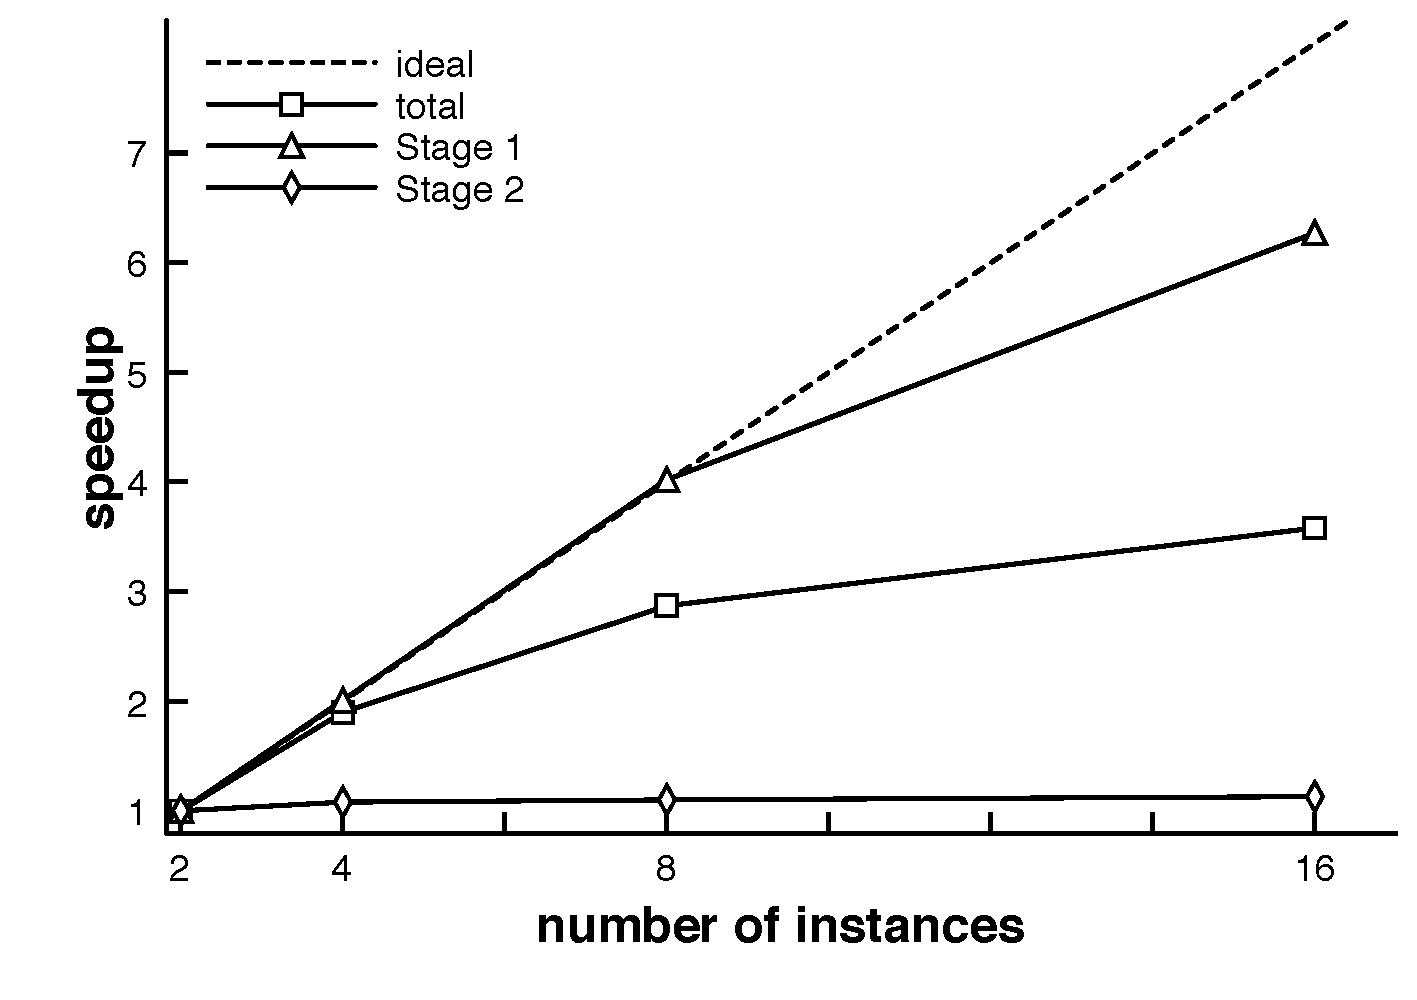
\includegraphics[width=\textwidth]{parma/speedup}
    \caption{Speedup analysis broken down by stages.}
    \label{fig:parmaspeedup}
  \end{subfigure}
  \hfill
  \begin{subfigure}[b]{0.49\textwidth}
    \centering
    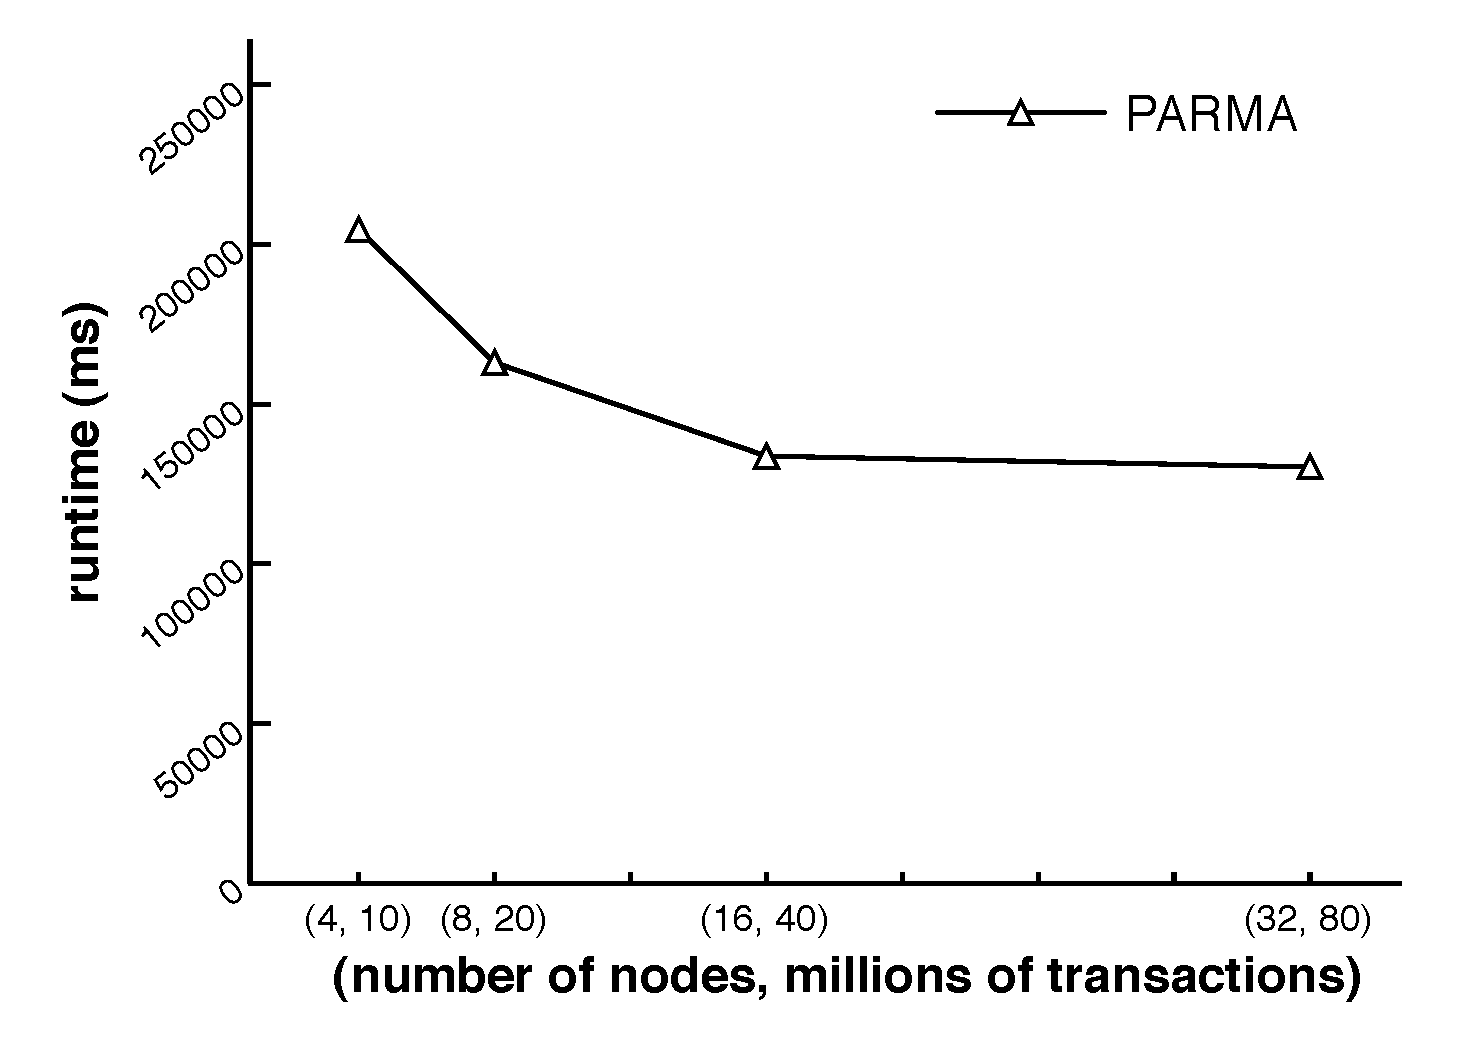
\includegraphics[width=\textwidth]{parma/scalability}
    \caption{Scalability as both data and cluster size are increased.}
    \label{fig:parmascalability}
  \end{subfigure}
  \caption{Speedup and scalability.}
\end{figure}

Also, as is clearly visible in the graph, the sub-ideal overall
speedup is due largely to the poor speedup of stage 2. Stage 2 is
bound almost entirely by the communication costs of transmitting the
local frequent itemsets from stage 1 to the reducers that will do the
aggregation. Because the amount of local frequent itemsets does not
change as more nodes are added, the communication for this stage does
not change. What does change is the number of itemsets each node must
aggregate. During the reduce phase, each node is assigned a set of
keys. All key/value pairs emitted from the map phase are sent to the
reducer assigned their respective key. The reducer is in charge of
aggregating the values and emitting one aggregate value per key assigned
to it. As more reducers are added to the cluster, each reducer will
have fewer keys assigned to it, and therefore must aggregate across
fewer values, resulting in faster aggregation. The small but existent positive
change in the line for stage 2 is a result of this slight speedup of the reduce
phase. 

Figure \ref{fig:parmascalability} depicts the scalability of PARMA as both
the size of the dataset (i.e. number of transactions) and the number of
nodes in the cluster are increased. The data and nodes are scaled
proportionally so that the ratio of data to nodes remains constant
across all experiments. This result shows that as nodes and data are
increased proportionally, the total runtime actually begins to decrease
for larger datasets. This is because as nodes are added to the cluster, the runtime of
the Stage 1 reducer (FIM) is decreased while the relative costs of
the Stage 1 mapper and Stage 2 remain the same. There is a leveling
off of the runtime between the 40M and 80M datasets, which can be
explained using Amdhal's law; because only portions of the algorithm
are parallelizable, there is a theoretical maximum speedup that is
possible. Still, the constant runtime as data is increased
demonstrates PARMA's potential scalability to real-world cluster and
dataset sizes. 

A very important aspect of PARMA that should be stressed again
here is that the size of the sample that will be mined does not depend
directly on size of the original database, but instead on the
confidence parameters $\varepsilon$ and $\delta$. From a practical
perspective, this means that assuming confidence parameters are
unchanged, larger and larger datasets can be mined with very little
increase in overall runtime (the added cost will only be the extra
time spent reading the larger dataset initially during
sampling). Because of this, clusters do not need to scale
with the data, and often a relatively modest cluster size will be
able to mine itemsets in a very reasonable time. 

\subsection{Accuracy}
The output of PARMA is a collection of frequent itemsets which approximates the
collection one can obtain by mining the entire dataset. Although our analysis
shows that PARMA offers solid guarantees in terms of accuracy of the output, we
conducted an extensive evaluation to assess the actual performances of PARMA in
practice, especially in relation to what can be analytically proved.

We compared the results obtained by PARMA with the exact collection of
itemsets from the entire dataset, for different values of the parameters
$\varepsilon$, $\delta$, and $\theta$, and for different datasets. A first important
result is that in all the runs, the collection computed by PARMA was indeed an
absolute $\varepsilon$-close approximation to the real one, i.e., all the properties from
Definition~\ref{def:parmaeapproxfi} were satisfied. This fact suggests that the confidence in
the result obtained by PARMA is actually greater than the level $1-\delta$
suggested by the analysis. This can be explained by considering that we had to
use potentially loose theoretical bounds in the analysis to make it tractable. 

Given that all real frequent itemsets were included in the output, we then
focused on how many itemsets with real frequency in the interval
$[\theta-\varepsilon,\theta)$ were included in the output. It is important to
notice that these itemsets would be \emph{acceptable} false positives, as
Definition~\ref{def:parmaeapproxfi} does not forbid them to be present in the output.
We stress again that the output of PARMA never contained \emph{non-acceptable}
false positives, i.e. itemsets with real frequency less than the minimum
frequency threshold $\theta$. The number of acceptable false positives included in the
output of PARMA depends on the distribution of the real frequencies in the
interval $[\theta-\varepsilon,\theta)$, so it should not be judged in absolute
terms. In Table~\ref{tab:falsepositives} we report, for various values of
$\theta$, the number of real frequent itemsets (i.e., with real frequency at
least $\theta$, the number of acceptable false positives (AFP) contained in the output
of PARMA, and the number of itemsets with real frequency in the interval
$[\theta-\varepsilon,\theta)$, i.e., the maximum number of acceptable false
positives that may be contained in the output of PARMA (Max AFP). These numbers
refers to a run of PARMA on (samples of) the 10M dataset, with
$\varepsilon=0.05$ and $\delta=0.01$. It is evident that PARMA does a very good
job in filtering out even acceptable false positives, especially at lower
frequencies, when their number increases. This is thanks to the fact that  an
itemset is included in the output of PARMA if and only if it appears in the
majority of the collections obtained in the first stage. Itemsets with real frequencies
in $[\theta-\varepsilon,\theta)$ are not very likely to be contained in many of
these collections.

\begin{table}
  \centering
  \begin{tabular}{cccc}
    \hline
    $\theta$ & Real FI's & Output AFP's & Max AFP's \\
    \hline
    $0.06$ & 11016 & 11797 & 201636 \\
    $0.09$ & 2116& 4216& 10723 \\
    $0.12$ & 1367& 335& 1452\\
    $0.15$ & 1053& 299& 415\\
    \hline
  \end{tabular}
  \caption{Acceptable False Positives in the output of PARMA}
  \label{tab:falsepositives}
\end{table}

We conducted an evaluation of the accuracy of two other components of the
output of PARMA, namely the estimated frequencies for the itemsets in the output
and the width of the confidence bounds for these estimations. In
Figure~\ref{fig:parmaabsfreqerr} we show the distribution of the absolute error in
the estimation, i.e. $|\tilde{f}(X)-f_\Ds(X)|$ for all itemsets $X$ in the
output of PARMA, as $\theta$ varies. The lower end of the ``whisker'' indicates the minimum error,
the lower bound of the box corresponds to the first quartile, the segment across
the box to the median, and the upper bound of the box to the third quartile. The
top end of the whisker indicates the maximum error, and the central diamond
shows the mean. This figure (and also Figure~\ref{fig:parmaconfintwidth}) shows the values
for a run of PARMA on samples of the 10M dataset, with $\varepsilon=0.05$ and
$\delta=0.01$. We can see that even the maximum values are one order of
magnitude smaller than the threshold of $0.05$ guaranteed by the analysis, and
many of the errors are two or more orders of magnitude smaller. It is also
possible to appreciate that the distribution of the error would be heavily concentrated in a
small interval if the maximum error were not so high, effectively an outlier.
The fact that the average and the median of the error, together with the entire ``box'' move down as the
minimum frequency threshold decrease can be explained by the fact that at lower
frequencies more itemsets are considered, and this makes the distribution less
susceptible to outliers. Not only this is a sign of the high level of accuracy
achieved by PARMA, but also of its being consistently accurate on
a very large portion of the output.

\begin{figure}[htb]
 \centering
    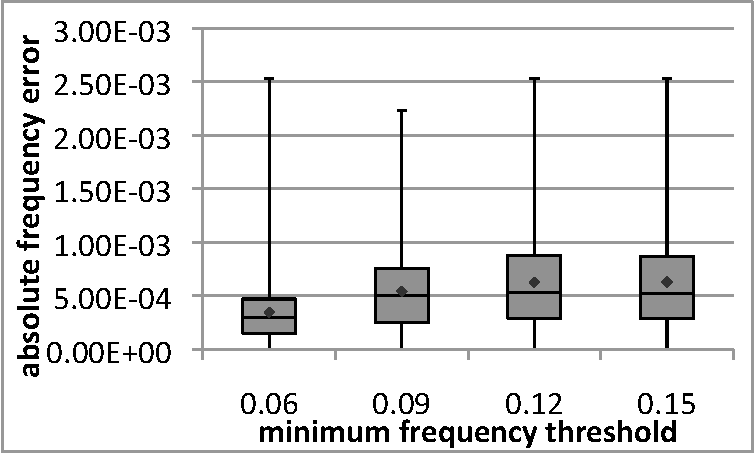
\includegraphics[width=0.75\textwidth]{parma/absfreqerr}
  \caption{Error in frequency estimations as frequency varies.}
  \label{fig:parmaabsfreqerr}
\end{figure}

\begin{figure}[htb]
 \centering
    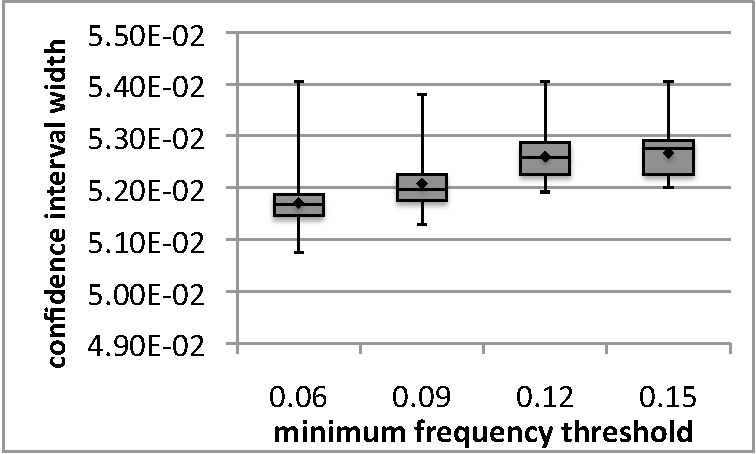
\includegraphics[width=0.75\textwidth]{parma/confintwidth}
  \caption{Width of the confidence intervals as frequency varies.}
  \label{fig:parmaconfintwidth}
\end{figure}

Finally, in Figure~\ref{fig:parmaconfintwidth} we show the distribution of the widths
of the confidence intervals $\mathcal{K}(A)$ for the frequency estimations
$\tilde{f}(A)$ of the itemsets $A$ in the output of PARMA. Given that
$\varepsilon=0.05$, the maximum allowed width was $2\varepsilon=0.1$. It is
evident from the figures that PARMA returns much narrower intervals, of size almost
$\varepsilon$. Moreover, the distribution of the width is very concentrated, as
shown by the small height of the boxes, suggesting that PARMA is extremely
consistent in giving very high quality confidence intervals for the estimations.
We state again that in all runs of PARMA in our tests, all the confidence
intervals contained the estimation and the real frequency, as requested by
Definition~\ref{def:parmaeapproxfi}. As seen in the case of the estimation
error, the distribution of the widths shifts down at lower thresholds $\theta$.
This is motivated by the higher number of itemsets in the output of PARMA at
those frequencies. Their presence makes the distribution more robust to
outliers. We can conclude that PARMA gives very narrow but
extremely accurate confidence intervals across the entirety of its output.

This analysis of the accuracy of various aspects of PARMA's output shows that
PARMA can be very useful in practice, and the confidence of the end user in
the collections of itemsets and estimations given in its output can be even higher
than what is guaranteed by the analysis.


\section{Conclusions}
\label{sec:parmaconc}

In this paper, we have described PARMA, a parallel algorithm for mining
quasi-optimal collections of frequent itemsets and association rules in MapReduce.
We showed through theoretical analysis that PARMA offers provable guarantees on
the quality of the output collections. Through experimentation on a wide range
of datasets ranging in size from 5 million to 50 million transactions,
we have demonstrated a 30-55\% runtime improvement over PFP, the
current state-of-the-art in exact parallel mining algorithms on MapReduce.
Empirically we were able to verify the accuracy of the theoretical bounds, as
well as show that in practice our results are orders of magnitude more accurate
than is analytically guaranteed. Thus PARMA is an algorithm that can scale to
arbitrary data sizes while simultaneously providing nearly perfect results. 

\section{Acknowledgments}
\label{sec:parmaack}
The work of Riondato, DeBrabant, and Upfal was supported in part by NSF award IIS-0905553.


%\bibliographystyle{abbrv}
%\bibliography{fim,mrfim,mr} 
\iffalse
\begin{thebibliography}{10}
\begin{small}

\vspace{7pt}
\bibitem{AgrawalIS93}
R.~Agrawal, T.~Imieli\'{n}ski, and A.~Swami.
\newblock Mining association rules between sets of items in large databases.
\newblock SIGMOD '93.

\bibitem{AgrawalS94}
R.~Agrawal and R.~Srikant.
\newblock Fast algorithms for mining association rules in large databases.
\newblock VLDB '94.

\bibitem{Mahout}
{Apache Mahout}.
\newblock \url{http://mahout.apache.org/}.

\bibitem{BuehrerPTKS07}
G.~Buehrer, S.~Parthasarathy, S.~Tatikonda, T.~Kurc, and J.~Saltz.
\newblock Toward terabyte pattern mining: an architecture-conscious solution.
\newblock PPoPP '07.

\bibitem{ChierichettiKT10}
F.~Chierichetti, R.~Kumar, and A.~Tomkins.
\newblock Max-cover in {Map-Reduce}.
\newblock WWW '10.

\bibitem{ChuKLYBNO06}
C.-T. Chu, S.~K. Kim, Y.-A. Lin, Y.~Yu, G.~R. Bradski, A.~Y. Ng, and
  K.~Olukotun.
\newblock {Map-Reduce} for machine learning on multicore.
\newblock NIPS '06.

\bibitem{Fp}
F.~Coenen.
%\newblock The {LUCS-KDD FP}-growth association rule mining algorithm.
\newblock
\url{http://www.cxc.liv.ac.uk/~frans/KDD/Software/FPgrowth/fpGrowth.html}

\bibitem{CongHHP05}
S.~Cong, J.~Han, J.~Hoeflinger, D.~Padua.
\newblock A sampling-based framework for parallel data mining.
\newblock PPoPP '05.

\bibitem{ARTool}
L.~Cristofor.
\newblock {ART}ool.
\newblock \url{http://www.cs.umb.edu/~laur/ARtool/}, 2006.

\bibitem{CryansRC10}
J.-D. Cryans, S.~Ratt{\'e}, and R.~Champagne.
\newblock Adaptation of {APriori} to {MapReduce} to build a warehouse of
  relations between named entities across the web.
\newblock DBKDA '10.

\bibitem{DeanG08}
J.~Dean and S.~Ghemawat.
\newblock {MapReduce}: Simplified data processing on large clusters.
\newblock {\em CACM}, 51(1):107--113, 2008.

\bibitem{EHZaiane06}
M.~El-Hajj and O.~Zaiane.
\newblock Parallel leap: large-scale maximal pattern mining in a distributed
  environment.
\newblock ICPADS '06.

\bibitem{FangEtAl08}
W.~Fang, K.~K. Lau, M.~Lu, X.~Xiao, C.~K. Lam, Y.~Yang, B.~He, Q.~Luo, P.~V.
  Sander, and K.~Yang.
\newblock Parallel data mining on graphics processors.
\newblock Technical Report~07, The Hong Kong University of Science {\&}
  Technology, 2008.

\bibitem{GhotingKPK11}
A.~Ghoting, P.~Kambadur, E.~Pednault, and R.~Kannan.
\newblock {NIMBLE}: a toolkit for the implementation of parallel data mining
and machine learning algorithms on {MapReduce}.
\newblock KDD '11.

\bibitem{GoodrichSZ11}
M.~T. Goodrich, N.~Sitchinava, and Q.~Zhang.
\newblock Sorting, searching, and simulation in the {MapReduce} framework.
\newblock {\em CoRR}, abs/1101.1902, 2011.

\bibitem{Hammoud11}
S.~Hammoud.
\newblock {\em MapReduce Network Enabled Algorithms for Classification Based on
  Association Rules}.
\newblock PhD thesis, Brunel University, 2011.

\bibitem{HanPY00}
J.~Han, J.~Pei, and Y.~Yin.
\newblock Mining frequent patterns without candidate generation.
\newblock {\em SIGMOD Rec.}, 29:1--12, May 2000.

\bibitem{LiWZZC08}
H.~Li, Y.~Wang, D.~Zhang, M.~Zhang, and E.~Y. Chang.
\newblock {PFP}: Parallel {FP-G}rowth for query recommendation.
\newblock RecSys '08.

\bibitem{LiZ11}
L.~Li and M.~Zhang.
\newblock The strategy of mining association rule based on cloud computing.
\newblock BCGIN '11.

\bibitem{LiG04}
Y.~Li and R.~Gopalan.
\newblock Effective sampling for mining association rules.
\newblock AI '04.

\bibitem{LinS10}
J.~Lin and M.~Schatz.
\newblock Design patterns for efficient graph algorithms in MapReduce.
\newblock  MLG '10.

\bibitem{LiuLZT07}
L.~Liu, E.~Li, Y.~Zhang, Z.~Tang.
\newblock Optimization of frequent itemset mining on multiple-core processor.
\newblock VLDB '07.

\bibitem{MannilaTV94}
H.~Mannila, H.~Toivonen, and I.~Verkamo.
\newblock Efficient algorithms for discovering association rules.
\newblock KDD '94.

\bibitem{MitzenmacherU05}
M.~Mitzenmacher and E.~Upfal.
\newblock {\em Probability and computing}.
\newblock Cambridge University Press, 2005.

\bibitem{OzkuralUA11}
E.~Ozkural, B.~Ucar, and C.~Aykanat.
\newblock Parallel frequent item set mining with selective item replication.
\newblock {\em IEEE Trans. on Paral. and Distrib. Sys.},
  22(10):1632--1640, 2011.

\bibitem{Parthasarathy02}
S.~Parthasarathy.
\newblock Efficient progressive sampling for association rules.
\newblock ICDM '02.

\bibitem{PietracaprinaPRSU11}
A.~Pietracaprina, G.~Pucci, M.~Riondato, F.~Silvestri, and E.~Upfal.
\newblock Space-round tradeoffs for {MapReduce} computations.
\newblock ICS' 12. 

\bibitem{PietracaprinaRUV10}
A.~Pietracaprina, M.~Riondato, E.~Upfal, and F.~Vandin.
\newblock Mining top-{K} frequent itemsets through progressive sampling.
\newblock {\em Data Min.~and Knowl.~Disc}, 21:310--326, 2010.

\bibitem{RiondatoU11}
M.~Riondato and E.~Upfal.
\newblock Efficient discovery of association rules and frequent itemsets
  through sampling with tight performance guarantees.
\newblock {\em CoRR}, abs/1111.6937v3, 2012.

\bibitem{JinYA05}
J.~Ruoming, Y.~Ge, and G.~Agrawal.
\newblock Shared memory parallelization of data mining algorithms: techniques,
  programming interface, and performance.
\newblock {\em IEEE Trans. on Knowl. and Data Engin.}, 17(1):71--89, 2005.

\bibitem{baron}
N.~V. Sahinidis and M.~Tawarmalani.
\newblock {\em {BARON 9.0.4: Global Optimization of Mixed-Integer Nonlinear
  Programs, {\em User's Manual}}}, 2010.

\bibitem{Toivonen96}
H.~Toivonen.
\newblock Sampling large databases for association rules.
\newblock VLDB '96.

\bibitem{YangLF10}
X.~Y. Yang, Z.~Liu, and Y.~Fu.
\newblock {MapReduce} as a programming model for association rules algorithm on
  {Hadoop}.
\newblock ICIS '10.

\bibitem{Zaki99}
M.~Zaki.
\newblock Parallel and distributed association mining: a survey.
\newblock {\em IEEE Concurrency}, 7(4):14 --25, 1999.

\bibitem{ZakiPLO97}
M.~Zaki, S.~Parthasarathy, W.~Li, and M.~Ogihara.
\newblock Evaluation of sampling for data mining of association rules.
\newblock RIDE '97.

\bibitem{ZhouZCLF10}
L.~Zhou, Z.~Zhong, J.~Chang, J.~Li, J.~Huang, and S.~Feng.
\newblock Balanced parallel {FP-Growth} with {MapReduce}.
\newblock YC-ICT '10.

\end{small}
\end{thebibliography}
\fi

